

\chapter{Simulation Based Inference}







\section{Simulation and Randomization with the  \texttt{mosaic} Package}

Software environments almost always provide an important feature:
\authNoted{Why use itemize when you want to enumerate?  If we don't like the 
display of enumerate, we should reset the defaults.  I'm switching to enumerate.
---rjp.  DTK says, ``Thanks.''  I didn't know about the saveenumi and
reuseenumi.  Very helpful.  One of many things I'm learning.  }
\begin{enumerate}
  \item They allow potentially complicated operations to be
    packaged with a simple interface, making them easy to use.
	\saveenumi
\end{enumerate}
An environment that is integrated with a programming language provides
an additional capability:
\begin{enumerate}
\reuseenumi
  \item New operations can be constructed from existing ones.
\end{enumerate}

Any proper statistics environment should offer the ease of use of
(1).  \R, like many packages, offers a large set of pre-packaged
operations.  But, as a modern programming language, \R\ offers the
advantage of making (2) available as well as (1).  In addition to
enabling \R\ to provide ready access to new forms of state-of-the-art
computing, the programming-language features of \R\ also enable the
operations in (1) to be de-constructed and presented to students in a
transparent and intelligible way that reveals the underlying logic.

One of the important goals of the \pkg{mosaic} package is to provide
elementary commands that can be easily strung together by novices
without having to master the esoteric aspects of programming.  
\FoodForThought[\centerline{Suggestion Box}]{We are interested in your 
feedback while we develop these tools.}%
This
chapter will describe a few such key operations and how they connect
to one another: random sampling and resampling, replication of random
trials, summarizing the results of multiple trials.  As you will see,
the \pkg{mosaic} operations allow students to implement each of the
operations in what George Cobb calls the ``3 Rs'' of statistical
inference: Randomization, Replication, and Rejection \cite{USCOTS-cobb-2005}.
By putting the 3 Rs together in various ways, students learn to
generalize and internalize the logic of inference, rather than just
following formulaic methods.  
More examples of the use of R as this sort
of \emph{sandbox} for experimentation can be found in \cite{hort:brow:2004}.

There's an interesting discussion of the role of simulation in \cite{speed:2011}, where
he notes the changing role of simulation.  It used to be:
\begin{quote}
something that people did when they can't do the math. $\ldots$ It now seems that we
are heading into an era when all statistical analysis can be done by simulation.
\end{quote}


\subsection{Sampling From Day 1 with \texttt{rflip()}}

Since tossing a coin is one of the most familiar examples of randomness, we've added to
\pkg{mosaic} a function that facilitates simulating coin tosses. 
\begin{knitrout}
\definecolor{shadecolor}{rgb}{.97, .97, .97}{\color{fgcolor}\begin{kframe}
\begin{flushleft}
\ttfamily\noindent
\hlfunctioncall{rflip}\hlkeyword{(}\hlnumber{20}\hlkeyword{)}\mbox{}
\normalfont
\end{flushleft}
\begin{verbatim}

Flipping 20 coins [ Prob(Heads) = 0.5 ] ...

T H T H H T H H H T H T H H T H T T T H

Result: 11 heads.

\end{verbatim}
\begin{flushleft}
\ttfamily\noindent
\hlfunctioncall{as.numeric}\hlkeyword{(}\hlfunctioncall{rflip}\hlkeyword{(}\hlnumber{20}\hlkeyword{)}\hlkeyword{)}{\ }{\ }\hlcomment{\usebox{\hlnormalsizeboxhash}{\ }just{\ }count{\ }how{\ }many{\ }heads}\mbox{}
\normalfont
\end{flushleft}
\begin{verbatim}
[1] 13
\end{verbatim}
\end{kframe}}
\end{knitrout}



In addition to the Lady Tasting Tea activity (Section~\ref{sec:lady-tasting-tea}),
other activities can be devised to help students develop a sense for randomness 
and variability.

\begin{enumerate}
\item If you flip a coin 100 times, how often will you get exactly 50 heads?
Between 45 and 55 heads?  Between 40 and 60 heads?
\item
If you flip a coin 20 times, how long is the longest run of either heads or tails typically?

This can be part of demonstration where you have students write down strings of H and T
that ``look random'' and another set based on actual coin tosses.  Then see if you can 
tell them which are which.

\item
\function{rflip()} allows you to flip biased coins as well.  Let's simulate a 90\%
free throw shooter shooting 10 free throws.
\begin{knitrout}
\definecolor{shadecolor}{rgb}{.97, .97, .97}{\color{fgcolor}\begin{kframe}
\begin{flushleft}
\ttfamily\noindent
\hlfunctioncall{rflip}\hlkeyword{(}\hlnumber{10}\hlkeyword{,}{\ }\hlargument{prob}{\ }\hlargument{=}{\ }\hlnumber{0.9}\hlkeyword{)}\mbox{}
\normalfont
\end{flushleft}
\begin{verbatim}

Flipping 10 coins [ Prob(Heads) = 0.9 ] ...

H H H H H H H H H H

Result: 10 heads.

\end{verbatim}
\end{kframe}}
\end{knitrout}


It's the end of the game.  Your team is down by one point.  Free Throw Freddie,
a 90\% free throw shooter, has been fouled while shooting.  What are the chances 
that your team wins (because Freddie makes 2 shots in a row), loses (because he misses 
both shots), or has to play an overtime period (because he makes one of the two)?

\begin{knitrout}
\definecolor{shadecolor}{rgb}{.97, .97, .97}{\color{fgcolor}\begin{kframe}
\begin{flushleft}
\ttfamily\noindent
\hlsymbol{simulated.shots}{\ }\hlassignement{\usebox{\hlnormalsizeboxlessthan}-}{\ }\hlfunctioncall{do}\hlkeyword{(}\hlnumber{2000}\hlkeyword{)}{\ }\hlkeyword{*}{\ }\hlfunctioncall{rflip}\hlkeyword{(}\hlnumber{2}\hlkeyword{,}{\ }\hlargument{prob}{\ }\hlargument{=}{\ }\hlnumber{0.9}\hlkeyword{)}\hspace*{\fill}\\
\hlstd{}\hlfunctioncall{with}\hlkeyword{(}\hlsymbol{simulated.shots}\hlkeyword{,}{\ }\hlfunctioncall{table}\hlkeyword{(}\hlsymbol{heads}\hlkeyword{)}\hlkeyword{)}\mbox{}
\normalfont
\end{flushleft}
\begin{verbatim}
heads
   0    1    2 
  14  371 1615 
\end{verbatim}
\end{kframe}}
\end{knitrout}


\item 
It can be fun to have students compare the results of flipping, spinning, and tipping pennies.
Many are surprised to learn that these do not all have same probability of producing heads.
\end{enumerate}

\authNote{Add some more of these.  Should we include examples where the coin is 
biased -- free throw shooting comes to mind, for example.  Also the tipping 
and spinning pennies activities.}%

\subsection{Sampling and Resampling}

Arguably, the most important operation in statistics is sampling:
ideally, selecting a random subset from a population.  Regrettably,
sampling takes work and time, so instructors tend to de-emphasize the
actual practice of sampling in favor of theoretical descriptions.
What's more, the algebraic notation in which much of conventional
textbook statistics is written does not offer an obvious notation for sampling.

With the computer, however, these efficiency and notation obstacles
can be overcome.  Sampling can be placed in its rightfully central
place among the statistical concepts in our courses.

In doing so, why not start right off with a sample from a population?
One example is the population of US states:

\authNoted{DTK: I'm reading it in this awkward way until I can add the dataset to
  the \pkg{mosaic} package.  In the \pkg{mosaic} package, the current ``SAT'' data
set has just one variable.  My view is that all such data sets should
be data frames.  But I understand the virtue of having a few that
students can use without the \$ notation.}%
\authNoted{RJP: I added the data and cleaned it up a bit.
All you need do is add documentation.}%

\begin{example}[ (Sampling from 50 States)]

Students in the US will know that there are 50 states:
\begin{knitrout}
\definecolor{shadecolor}{rgb}{.97, .97, .97}{\color{fgcolor}\begin{kframe}
\begin{flushleft}
\ttfamily\noindent
\hlfunctioncall{nrow}\hlkeyword{(}\hlsymbol{SAT}\hlkeyword{)}{\ }{\ }\hlcomment{\usebox{\hlnormalsizeboxhash}{\ }SAT{\ }is{\ }a{\ }data{\ }frame{\ }in{\ }the{\ }mosaic{\ }package}\mbox{}
\normalfont
\end{flushleft}
\begin{verbatim}
[1] 50
\end{verbatim}
\end{kframe}}
\end{knitrout}




One of the variables to be measured from the population is the
student/teacher ratio.  There are two equivalent ways to calculate this quantity:
\begin{knitrout}
\definecolor{shadecolor}{rgb}{.97, .97, .97}{\color{fgcolor}\begin{kframe}
\begin{flushleft}
\ttfamily\noindent
\hlfunctioncall{mean}\hlkeyword{(}\hlsymbol{SAT}\hlkeyword{\usebox{\hlnormalsizeboxdollar}}\hlsymbol{ratio}\hlkeyword{)}\mbox{}
\normalfont
\end{flushleft}
\begin{verbatim}
 mean 
16.86 
\end{verbatim}
\end{kframe}}
\end{knitrout}


\authNoted{DTK: There's another style that we could push.  I'm
  interested in your reaction to it. This has the advantage of segregating the
  randomization part from the calculation part.  
  I'll try using this style in the following, and we
can easily change back to a more conventional style if it gets irritating.}

\begin{knitrout}
\definecolor{shadecolor}{rgb}{.97, .97, .97}{\color{fgcolor}\begin{kframe}
\begin{flushleft}
\ttfamily\noindent
\hlfunctioncall{with}\hlkeyword{(}\hlsymbol{SAT}\hlkeyword{,}{\ }\hlfunctioncall{mean}\hlkeyword{(}\hlsymbol{ratio}\hlkeyword{)}\hlkeyword{)}\mbox{}
\normalfont
\end{flushleft}
\begin{verbatim}
 mean 
16.86 
\end{verbatim}
\end{kframe}}
\end{knitrout}


Every student who does this calculation will get the same result.
But if each student takes a random sample (without replacement) of, say, 4 states:
\authNoted{RJP: If we want a sample, let's call it a sample, not a shuffle.  I've changed
the \R\ code throughout this section.}%
\begin{knitrout}
\definecolor{shadecolor}{rgb}{.97, .97, .97}{\color{fgcolor}\begin{kframe}
\begin{flushleft}
\ttfamily\noindent
\hlfunctioncall{sample}\hlkeyword{(}\hlsymbol{SAT}\hlkeyword{,}{\ }\hlnumber{4}\hlkeyword{)}\mbox{}
\normalfont
\end{flushleft}
\begin{verbatim}
       state expend ratio salary frac verbal math  sat orig.ids
20  Maryland  7.245  17.0  40.66   64    430  479  909       20
15      Iowa  5.483  15.8  31.51    5    516  583 1099       15
23 Minnesota  6.000  17.5  35.95    9    506  579 1085       23
35      Ohio  6.162  16.6  36.80   23    460  515  975       35
\end{verbatim}
\end{kframe}}
\end{knitrout}


Then each student gets a potentially different result.

Doing this with a classroom of students will immediately elicit a
realization that the random sample is exactly that.  Ask the class:
Who got California?  (There should be one or two in a class of 20.)
Who got Alabama?  Did anyone get the same state twice?
\authNote{RJP:
No one will get the same state twice with \texttt{smaple()} or 
with \texttt{shuffle()} under the default settings.  \texttt{resample()} 
on the other hand, samples with replacement by default.
We could use \texttt{deal()} here, but why mix metaphors when you are talking
about sampling?
}
\end{example}

\authNote{We had \texttt{echo=FALSE} here, but I think we mean \texttt{eval=FALSE} ---rjp}%
\begin{problem}
 (This isn't a question for beginning students, just one
for developing instructor capabilities.)  
How would you demonstrate that there are 50
different states, rather than just 50 cases that might include
duplicates?  
Try each of the following
and see if you can understand what's going on in each of them:
\begin{knitrout}
\definecolor{shadecolor}{rgb}{.97, .97, .97}{\color{fgcolor}\begin{kframe}
\begin{flushleft}
\ttfamily\noindent
\hlfunctioncall{with}\hlkeyword{(}\hlsymbol{SAT}\hlkeyword{,}{\ }\hlfunctioncall{table}\hlkeyword{(}\hlsymbol{state}\hlkeyword{)}\hlkeyword{)}\hspace*{\fill}\\
\hlstd{}\hlfunctioncall{length}\hlkeyword{(}\hlfunctioncall{with}\hlkeyword{(}\hlsymbol{SAT}\hlkeyword{,}{\ }\hlfunctioncall{table}\hlkeyword{(}\hlsymbol{state}\hlkeyword{)}\hlkeyword{)}\hlkeyword{)}\hspace*{\fill}\\
\hlstd{}\hlfunctioncall{with}\hlkeyword{(}\hlsymbol{SAT}\hlkeyword{,}{\ }\hlfunctioncall{table}\hlkeyword{(}\hlfunctioncall{table}\hlkeyword{(}\hlsymbol{state}\hlkeyword{)}\hlkeyword{)}\hlkeyword{)}\hspace*{\fill}\\
\hlstd{}\hlfunctioncall{table}\hlkeyword{(}\hlfunctioncall{table}\hlkeyword{(}\hlsymbol{SAT}\hlkeyword{\usebox{\hlnormalsizeboxdollar}}\hlsymbol{state}\hlkeyword{)}\hlkeyword{)}\mbox{}
\normalfont
\end{flushleft}
\end{kframe}}
\end{knitrout}

\end{problem}

The value of some measure for the population is, of course, called the 
\term{population parameter}.  
\authNoted{RJP: Why use scare quotes here?  Use \texttt{\term{}} to highlight terms.  We 
can define that to be boldface font or some such.}%
But for a sample, it's a \term{sample statistic}.  It's
worthwhile to make the distinction concrete:
\begin{knitrout}
\definecolor{shadecolor}{rgb}{.97, .97, .97}{\color{fgcolor}\begin{kframe}
\begin{flushleft}
\ttfamily\noindent
\hlfunctioncall{with}\hlkeyword{(}\hlsymbol{SAT}\hlkeyword{,}{\ }\hlfunctioncall{mean}\hlkeyword{(}\hlsymbol{ratio}\hlkeyword{)}\hlkeyword{)}{\ }{\ }\hlcomment{\usebox{\hlnormalsizeboxhash}{\ }population{\ }parameter}\mbox{}
\normalfont
\end{flushleft}
\begin{verbatim}
 mean 
16.86 
\end{verbatim}
\begin{flushleft}
\ttfamily\noindent
\hlfunctioncall{with}\hlkeyword{(}\hlfunctioncall{sample}\hlkeyword{(}\hlsymbol{SAT}\hlkeyword{,}{\ }\hlnumber{4}\hlkeyword{)}\hlkeyword{,}{\ }\hlfunctioncall{mean}\hlkeyword{(}\hlsymbol{ratio}\hlkeyword{)}\hlkeyword{)}{\ }{\ }\hlcomment{\usebox{\hlnormalsizeboxhash}{\ }statistic{\ }from{\ }a{\ }sample{\ }of{\ }4{\ }states}\mbox{}
\normalfont
\end{flushleft}
\begin{verbatim}
mean 
16.4 
\end{verbatim}
\end{kframe}}
\end{knitrout}


Good questions to ask in class at this point: Who got a sample
statistic that's bigger than the population parameter?  (About half
the class will say yes.)  Who got a sample statistic that's exactly
equal to the population parameter?  (It's unlikely that there will be a match.)
\authNoted{Is it worth the effort to write a few macros that place marginal
notes alerting the reader to things like ``questions for students'', 
``just for instructors'', ``R pitfalls'', etc.  
Perhaps we could use the data set identifier from Danny's book
as a model?  I'm thinking it would be nice to make it easier for users to locate
various types of material.}


At this point, it's helpful to point out that the reason we take
samples is because it can be difficult or impossible to measure every
member of the population.  Of course, it's not so difficult if your
population is the 50 US States, but what if your population were the
all people living in the US: that's over 300,000,000 people!  


\subsection{Taking Randomness Seriously}

\label{sec:taking-randomness-seriously}

It's tempting to think that ``random'' means that anything goes.  This
is, after all, the everyday meaning of the word.  In statistics,
though, the point of randomness is to get a representative sample, or
to assign experimental treatments in some fairly even way.   
\authNote{RJP: 'fairly even' is pretty vague and potentially misleading.
Randomness is really about having some knowledge about the variability.
Other methods may have less variability, but if we don't know how to quantify it
and if it is miscentered (biased), it doesn't do us any good. }%
Using
randomness properly means taking care and being formal about where the
randomness comes from.  When you finally submit the research paper you
have written after your long years of labor, you don't want it to be
rejected because the reviewer isn't convinced that what you called
``random'' was really so.

First, to demonstrate that the sort of computer-generated random
sampling produces reasonable results.  Perhaps it's a little too early
in the course to talk about sampling distributions, but you certainly
can have your class generate random samples of a reasonable size and
show that sample statistics are reasonably close to the population parameter.  
\authNote{RJP: samples are not close to parameters, statistics are.  I changed
'they' to 'sample statistics'}%
For
instance, have each student in your class do this:
\begin{knitrout}
\definecolor{shadecolor}{rgb}{.97, .97, .97}{\color{fgcolor}\begin{kframe}
\begin{flushleft}
\ttfamily\noindent
\hlfunctioncall{with}\hlkeyword{(}\hlsymbol{SAT}\hlkeyword{,}{\ }\hlfunctioncall{mean}\hlkeyword{(}\hlsymbol{ratio}\hlkeyword{)}\hlkeyword{)}\mbox{}
\normalfont
\end{flushleft}
\begin{verbatim}
 mean 
16.86 
\end{verbatim}
\begin{flushleft}
\ttfamily\noindent
\hlfunctioncall{with}\hlkeyword{(}\hlfunctioncall{sample}\hlkeyword{(}\hlsymbol{SAT}\hlkeyword{,}{\ }\hlnumber{25}\hlkeyword{)}\hlkeyword{,}{\ }\hlfunctioncall{mean}\hlkeyword{(}\hlsymbol{ratio}\hlkeyword{)}\hlkeyword{)}\mbox{}
\normalfont
\end{flushleft}
\begin{verbatim}
 mean 
16.71 
\end{verbatim}
\end{kframe}}
\end{knitrout}

Or, each student can do this several times:
\FoodForThought[\centerline{To Do}]{We'll have more to say about \function{do()} shortly.}%
\begin{knitrout}
\definecolor{shadecolor}{rgb}{.97, .97, .97}{\color{fgcolor}\begin{kframe}
\begin{flushleft}
\ttfamily\noindent
\hlfunctioncall{do}\hlkeyword{(}\hlnumber{5}\hlkeyword{)}{\ }\hlkeyword{*}{\ }\hlfunctioncall{with}\hlkeyword{(}\hlfunctioncall{sample}\hlkeyword{(}\hlsymbol{SAT}\hlkeyword{,}{\ }\hlnumber{25}\hlkeyword{)}\hlkeyword{,}{\ }\hlfunctioncall{mean}\hlkeyword{(}\hlsymbol{ratio}\hlkeyword{)}\hlkeyword{)}\mbox{}
\normalfont
\end{flushleft}
\begin{verbatim}
   mean
1 16.50
2 16.37
3 17.32
4 16.73
5 16.14
\end{verbatim}
\end{kframe}}
\end{knitrout}

This raises the question, naturally enough, of what ``reasonably
close'' means, and what it means to measure ``how close.''
Eventually, that might lead you into consideration of differences,
mean differences, mean square differences, and root mean square
differences: the standard deviation and variance.  But even before
encountering this formality the
students should be able to see that there is nothing systematically
wrong with the answers they get from their random samples.  Some are too high compared to the
population parameter, some are too low, but as a group they are pretty
well centered.

For some applications it is useful to have an alternative vocabulary.  If you are fond
of examples involving cards, you can use \function{deal()} and \function{shuffle()}
instead of \function{sample()}.
\begin{knitrout}
\definecolor{shadecolor}{rgb}{.97, .97, .97}{\color{fgcolor}\begin{kframe}
\begin{flushleft}
\ttfamily\noindent
\hlcomment{\usebox{\hlnormalsizeboxhash}{\ }These{\ }are{\ }equivalent}\hspace*{\fill}\\
\hlstd{}\hlfunctioncall{sample}\hlkeyword{(}\hlsymbol{cards}\hlkeyword{,}{\ }\hlnumber{5}\hlkeyword{)}\mbox{}
\normalfont
\end{flushleft}
\begin{verbatim}
[1] "JD" "3D" "3C" "2H" "4D"
\end{verbatim}
\begin{flushleft}
\ttfamily\noindent
\hlfunctioncall{deal}\hlkeyword{(}\hlsymbol{cards}\hlkeyword{,}{\ }\hlnumber{5}\hlkeyword{)}\mbox{}
\normalfont
\end{flushleft}
\begin{verbatim}
[1] "AD" "4S" "QC" "6C" "AH"
\end{verbatim}
\end{kframe}}
\end{knitrout}

\begin{knitrout}
\definecolor{shadecolor}{rgb}{.97, .97, .97}{\color{fgcolor}\begin{kframe}
\begin{flushleft}
\ttfamily\noindent
\hlcomment{\usebox{\hlnormalsizeboxhash}{\ }These{\ }are{\ }equivalent}\hspace*{\fill}\\
\hlstd{}\hlfunctioncall{sample}\hlkeyword{(}\hlsymbol{cards}\hlkeyword{)}\mbox{}
\normalfont
\end{flushleft}
\begin{verbatim}
 [1] "JC"  "3S"  "3C"  "4S"  "2S"  "5S"  "6D"  "2D"  "KS"  "7S"  "AH"  "KD"  "QD"  "4H"  "4D"  "9S" 
[17] "KH"  "KC"  "10S" "10C" "3H"  "JS"  "QH"  "2C"  "2H"  "10H" "10D" "AC"  "7H"  "5C"  "QS"  "5H" 
[33] "9C"  "6H"  "AD"  "3D"  "9H"  "7D"  "QC"  "5D"  "8D"  "4C"  "8C"  "7C"  "6C"  "8S"  "9D"  "AS" 
[49] "6S"  "JH"  "JD"  "8H" 
\end{verbatim}
\begin{flushleft}
\ttfamily\noindent
\hlfunctioncall{shuffle}\hlkeyword{(}\hlsymbol{cards}\hlkeyword{)}\mbox{}
\normalfont
\end{flushleft}
\begin{verbatim}
 [1] "2H"  "QD"  "AS"  "9H"  "10S" "7S"  "6S"  "6H"  "8H"  "4S"  "10C" "3H"  "5C"  "8D"  "4H"  "2C" 
[17] "7C"  "2S"  "3S"  "AC"  "9D"  "KS"  "9C"  "QC"  "JC"  "AH"  "3D"  "10H" "5H"  "JS"  "KC"  "8S" 
[33] "8C"  "QS"  "5D"  "JD"  "6D"  "KD"  "JH"  "5S"  "6C"  "2D"  "3C"  "10D" "9S"  "QH"  "4C"  "4D" 
[49] "KH"  "7D"  "7H"  "AD" 
\end{verbatim}
\end{kframe}}
\end{knitrout}


And for sampling with replacement, we offer \function{resample()}:
\begin{knitrout}
\definecolor{shadecolor}{rgb}{.97, .97, .97}{\color{fgcolor}\begin{kframe}
\begin{flushleft}
\ttfamily\noindent
\hlcomment{\usebox{\hlnormalsizeboxhash}{\ }These{\ }are{\ }equivalent}\hspace*{\fill}\\
\hlstd{}\hlfunctioncall{sample}\hlkeyword{(}\hlnumber{1}\hlkeyword{:}\hlnumber{10}\hlkeyword{,}{\ }\hlnumber{5}\hlkeyword{,}{\ }\hlargument{replace}{\ }\hlargument{=}{\ }\hlnumber{TRUE}\hlkeyword{)}\mbox{}
\normalfont
\end{flushleft}
\begin{verbatim}
[1]  3  4  5  5 10
\end{verbatim}
\begin{flushleft}
\ttfamily\noindent
\hlfunctioncall{resample}\hlkeyword{(}\hlnumber{1}\hlkeyword{:}\hlnumber{10}\hlkeyword{,}{\ }\hlnumber{5}\hlkeyword{)}\mbox{}
\normalfont
\end{flushleft}
\begin{verbatim}
[1] 7 4 9 4 7
\end{verbatim}
\end{kframe}}
\end{knitrout}


\subsection{Illuminating Sampling Mistakes}
\authNote{RJP: The word 'illuminating' has two meanings intentionally -- but feel free to 
change if that's too cute.}%
It's helpful at this point to have some examples where an informal or careless
approach to randomness leads to misleading results.

Here are some that can be visually compelling:
\begin{enumerate}
\item Select books off a library shelf and count how many pages 
are in each book.
  When students pick books haphazardly, they get a systematic
  over-estimate of the page length.  
  
  A random sample of 25 is
  sufficient to see this for the large majority of students in the
  class.  Going up to 50, though tedious, makes the result even more compelling.
  \authNote{RJP:  I moved Danny's comment (Introduce the R app that let's
  students do this with the mouse.)  to this note.  
  It's too late in the game to put hard to spot cruft into the document
  that we need to remember to remove later.}%
  
\item A simulation of a real-world study of Alzheimer's disease.  The
  sampling process was to go to nursing homes on a given day and
  randomly pick out patients who were diagnosed with Alzheimer's.
  Their files were flagged and, after a few years, the data were
  examined to find the mean survival time, from when they entered the
  nursing home to when they died.  
  
\authNote{We can easily write an app that generates admission and
  death dates as Julian dates, and let's the student pick a random day
  of the year for the sampling.  A graphic shows how the random day
  tends to select those who are at the nursing home for a long time,
  rather than equally picking all patients.  Students can then compare
  the mean for the population to the mean for their haphazard sample.}%

  \item Sample people and find out how many siblings are in their family
  (including themselves).
  Use this data to estimate family size.  Since larger families have more
  children, we will over-sample larger families and over-estimate 
  family size.  Section~\ref{sec:fake-families} demonstrates how
  to fake a data set for this activity.  But for the present, we can
  use the \texttt{Galton} dataset and pretend to take a sample of,
  say, size 300 kids from the whole group of children that Galton had assembled.  
 
\begin{knitrout}
\definecolor{shadecolor}{rgb}{.97, .97, .97}{\color{fgcolor}\begin{kframe}
\begin{flushleft}
\ttfamily\noindent
\hlfunctioncall{data}\hlkeyword{(}\hlsymbol{Galton}\hlkeyword{)}\hspace*{\fill}\\
\hlstd{}\hlfunctioncall{with}\hlkeyword{(}\hlfunctioncall{sample}\hlkeyword{(}\hlsymbol{Galton}\hlkeyword{,}{\ }\hlnumber{300}\hlkeyword{)}\hlkeyword{,}{\ }\hlfunctioncall{mean}\hlkeyword{(}\hlsymbol{nkids}\hlkeyword{)}\hlkeyword{)}\mbox{}
\normalfont
\end{flushleft}
\begin{verbatim}
 mean 
6.237 
\end{verbatim}
\begin{flushleft}
\ttfamily\noindent
\hlfunctioncall{with}\hlkeyword{(}\hlfunctioncall{sample}\hlkeyword{(}\hlsymbol{Galton}\hlkeyword{,}{\ }\hlnumber{300}\hlkeyword{)}\hlkeyword{,}{\ }\hlfunctioncall{mean}\hlkeyword{(}\hlsymbol{nkids}\hlkeyword{)}\hlkeyword{)}\mbox{}
\normalfont
\end{flushleft}
\begin{verbatim}
mean 
6.16 
\end{verbatim}
\begin{flushleft}
\ttfamily\noindent
\hlfunctioncall{do}\hlkeyword{(}\hlnumber{5}\hlkeyword{)}{\ }\hlkeyword{*}{\ }\hlfunctioncall{with}\hlkeyword{(}\hlfunctioncall{sample}\hlkeyword{(}\hlsymbol{Galton}\hlkeyword{,}{\ }\hlnumber{300}\hlkeyword{)}\hlkeyword{,}{\ }\hlfunctioncall{mean}\hlkeyword{(}\hlsymbol{nkids}\hlkeyword{)}\hlkeyword{)}\mbox{}
\normalfont
\end{flushleft}
\begin{verbatim}
   mean
1 6.070
2 6.150
3 6.177
4 6.110
5 6.033
\end{verbatim}
\end{kframe}}
\end{knitrout}

The samples all give about the same answer: about 6 kids in a family.
But this is misleading!  The case in the \texttt{Galton} data is a
child, and families with more children have their family size
represented proportionally more.  


\authNote{DTK: To be added to the style guidelines????  
I like to have a macro that typesets variable names in
  a consistent way, e.g., a sans-serif font.  It doesn't matter so
  much what the typestyle is, so long as we can be consistent.  I
  suggest \texttt{\VN{}} as the markup.  We need a similar markup for
  data sets and for operators (so that we can make an index of operators.}
There are several ways to convert the \texttt{Galton} to a new data
set where the case is a family.  The key information is contained in
the \VN{family} variable, which has a unique value for each family.
The \texttt{duplicated} function identifies levels that are repeats of
earlier ones and so the following will do the job (although is not
necessarily something that you want to push onto students):
\begin{knitrout}
\definecolor{shadecolor}{rgb}{.97, .97, .97}{\color{fgcolor}\begin{kframe}
\begin{flushleft}
\ttfamily\noindent
\hlsymbol{families}{\ }\hlassignement{=}{\ }\hlfunctioncall{subset}\hlkeyword{(}\hlsymbol{Galton}\hlkeyword{,}{\ }\hlkeyword{!}\hlfunctioncall{duplicated}\hlkeyword{(}\hlsymbol{family}\hlkeyword{)}\hlkeyword{)}\mbox{}
\normalfont
\end{flushleft}
\end{kframe}}
\end{knitrout}

Of course, you will want to show that this has done the right job.  Compare
\begin{knitrout}
\definecolor{shadecolor}{rgb}{.97, .97, .97}{\color{fgcolor}\begin{kframe}
\begin{flushleft}
\ttfamily\noindent
\hlfunctioncall{nrow}\hlkeyword{(}\hlsymbol{families}\hlkeyword{)}\mbox{}
\normalfont
\end{flushleft}
\begin{verbatim}
[1] 197
\end{verbatim}
\end{kframe}}
\end{knitrout}

to 
\begin{knitrout}
\definecolor{shadecolor}{rgb}{.97, .97, .97}{\color{fgcolor}\begin{kframe}
\begin{flushleft}
\ttfamily\noindent
\hlfunctioncall{length}\hlkeyword{(}\hlfunctioncall{with}\hlkeyword{(}\hlsymbol{Galton}\hlkeyword{,}{\ }\hlfunctioncall{unique}\hlkeyword{(}\hlsymbol{family}\hlkeyword{)}\hlkeyword{)}\hlkeyword{)}\mbox{}
\normalfont
\end{flushleft}
\begin{verbatim}
[1] 197
\end{verbatim}
\end{kframe}}
\end{knitrout}


Now check out the average family size when the average is across
families, not across kids in families:
\begin{knitrout}
\definecolor{shadecolor}{rgb}{.97, .97, .97}{\color{fgcolor}\begin{kframe}
\begin{flushleft}
\ttfamily\noindent
\hlfunctioncall{with}\hlkeyword{(}\hlsymbol{families}\hlkeyword{,}{\ }\hlfunctioncall{mean}\hlkeyword{(}\hlsymbol{nkids}\hlkeyword{)}\hlkeyword{)}\mbox{}
\normalfont
\end{flushleft}
\begin{verbatim}
 mean 
4.563 
\end{verbatim}
\end{kframe}}
\end{knitrout}



  (Note:  In a higher-level course, you could ask students
  to determine a method to correct for this bias.)
\authNote{Consider whether my little example is too advanced and
  should be moved to a higher-level course.  A good general policy for
  this workshop would be to ask the users to mark up places where the
  commands seem too difficult, or to highlight ``student use'' versus
  ``instructor demonstration.''  There are always students who are
  keen to see more, even if they aren't expected to master it.}

  \authNote{RJP:  build appropriate data frames for this and Alzheimer's examples.
  Do we want to show how to build these?  I say yes.  It would be good for instructors
  to see how these are built.  Those who are not interested can simply
  copy.  We can put this stuff into a \texttt{demo()} for easy access.
  DTK: I agree.
  }

  \item
  Using \function{googleMap()} (see Section~\ref{sec:googleMap}) 
  we can compare uniform sampling of longitude 
  and latitude with correct sampling that takes into account that the earth
  is a sphere, not a cylinder.
\end{enumerate}

In each of these cases, follow up the haphazard or systematically biased 
sample with a formally generated sample (which is faster to do, in any event) and show that
the formally generated sample gives results that are more
representative of the population than the haphazardly sampled data.



%\subsection{Basic Sampling With \texttt{sample()}, \texttt{resample()}, and Cousins}

\subsection{Sampling from Distributions}

Later in the course, if you cover modeling with distributions, you can sample from 
these distributions instead of from data sets (treated like populations).
\R\ includes set of functions beginning with the letter \code{r} followed by the (abbreviated)
name of a family of distributions (see 
Table \ref{core:dist} in section \ref{sec:probability} for a list of probability distributions
available within base \R).  These functions all generate
a random sample from the distribution given a sample size and any necessary parameters 
for the distribution.

\begin{knitrout}
\definecolor{shadecolor}{rgb}{.97, .97, .97}{\color{fgcolor}\begin{kframe}
\begin{flushleft}
\ttfamily\noindent
\hlfunctioncall{rnorm}\hlkeyword{(}\hlnumber{20}\hlkeyword{,}{\ }\hlargument{mean}{\ }\hlargument{=}{\ }\hlnumber{500}\hlkeyword{,}{\ }\hlargument{sd}{\ }\hlargument{=}{\ }\hlnumber{100}\hlkeyword{)}{\ }{\ }\hlcomment{\usebox{\hlnormalsizeboxhash}{\ }fake{\ }SAT{\ }scores}\mbox{}
\normalfont
\end{flushleft}
\begin{verbatim}
 [1] 366.4 366.4 416.0 540.6 506.8 452.2 621.2 443.0 541.2 533.2 611.7 606.0 593.6 420.5 513.7 438.9
[17] 353.4 531.8 535.3 367.4
\end{verbatim}
\begin{flushleft}
\ttfamily\noindent
\hlfunctioncall{rexp}\hlkeyword{(}\hlnumber{20}\hlkeyword{,}{\ }\hlargument{rate}{\ }\hlargument{=}{\ }\hlnumber{1}\hlkeyword{/}\hlnumber{5}\hlkeyword{)}{\ }{\ }\hlcomment{\usebox{\hlnormalsizeboxhash}{\ }fake{\ }lifetime{\ }data}\mbox{}
\normalfont
\end{flushleft}
\begin{verbatim}
 [1]  0.5450  3.3602  3.4503  6.0536  1.8180  3.9899  3.2488  4.2669 11.6448  5.2622  7.4161  1.8058
[13]  5.0144  0.8469  1.6869  2.9181  4.3581  5.0110  0.2643  0.3542
\end{verbatim}
\begin{flushleft}
\ttfamily\noindent
\hlfunctioncall{rbinom}\hlkeyword{(}\hlnumber{20}\hlkeyword{,}{\ }\hlnumber{10}\hlkeyword{,}{\ }\hlnumber{0.5}\hlkeyword{)}{\ }{\ }\hlcomment{\usebox{\hlnormalsizeboxhash}{\ }how{\ }many{\ }heads{\ }in{\ }10{\ }coin{\ }tosses?}\mbox{}
\normalfont
\end{flushleft}
\begin{verbatim}
 [1] 6 6 1 6 4 7 5 3 4 6 5 6 4 5 6 6 4 3 5 5
\end{verbatim}
\begin{flushleft}
\ttfamily\noindent
\hlfunctioncall{rgeom}\hlkeyword{(}\hlnumber{20}\hlkeyword{,}{\ }\hlnumber{0.1}\hlkeyword{)}{\ }{\ }\hlcomment{\usebox{\hlnormalsizeboxhash}{\ }how{\ }long{\ }until{\ }Freddy{\ }misses{\ }his{\ }next{\ }free{\ }throw?}\mbox{}
\normalfont
\end{flushleft}
\begin{verbatim}
 [1] 29  0 15  7  2  7  0  3  5  2  5  3  1  0  1  1  1 11  4  0
\end{verbatim}
\end{kframe}}
\end{knitrout}


The \pkg{mosaic} package offers \function{rdata()} as an alternative to 
\function{resample()} with syntax that mirrors these functions for sampling from
a distribution.

\begin{knitrout}
\definecolor{shadecolor}{rgb}{.97, .97, .97}{\color{fgcolor}\begin{kframe}
\begin{flushleft}
\ttfamily\noindent
\hlfunctioncall{rdata}\hlkeyword{(}\hlnumber{20}\hlkeyword{,}{\ }\hlnumber{1}\hlkeyword{:}\hlnumber{4}\hlkeyword{)}{\ }{\ }\hlcomment{\usebox{\hlnormalsizeboxhash}{\ }samples{\ }with{\ }replacement}\mbox{}
\normalfont
\end{flushleft}
\begin{verbatim}
 [1] 4 3 1 4 4 4 2 2 2 1 3 2 1 1 2 2 3 2 2 1
\end{verbatim}
\end{kframe}}
\end{knitrout}


\begin{knitrout}
\definecolor{shadecolor}{rgb}{.97, .97, .97}{\color{fgcolor}\begin{kframe}
\begin{flushleft}
\ttfamily\noindent
\hlfunctioncall{set.seed}\hlkeyword{(}\hlnumber{123}\hlkeyword{)}\mbox{}
\normalfont
\end{flushleft}
\end{kframe}}
\end{knitrout}

\begin{knitrout}
\definecolor{shadecolor}{rgb}{.97, .97, .97}{\color{fgcolor}\begin{kframe}
\begin{flushleft}
\ttfamily\noindent
\hlcomment{\usebox{\hlnormalsizeboxhash}{\ }these{\ }are{\ }equivalent;{\ }{\ }note{\ }the{\ }order{\ }of{\ }the{\ }arguments.}\hspace*{\fill}\\
\hlstd{}\hlfunctioncall{resample}\hlkeyword{(}\hlsymbol{HELP}\hlkeyword{,}{\ }\hlnumber{2}\hlkeyword{)}\mbox{}
\normalfont
\end{flushleft}
\begin{verbatim}
    age anysubstatus anysub cesd d1 daysanysub dayslink drugrisk e2b female  sex g1b homeless i1
131  49            1    yes   22  5          1      126        0   4      0 male yes homeless 64
358  36            1    yes   36  3          3      362        0  NA      0 male  no   housed 25
     i2  id indtot linkstatus link   mcs   pcs pss_fr racegrp satreat sexrisk substance treat
131 179 144     42          1  yes 45.49 38.14      5   black      no       6   alcohol   yes
358  42 430     37          0   no 45.86 14.07      8   white      no       4   alcohol    no
\end{verbatim}
\begin{flushleft}
\ttfamily\noindent
\hlfunctioncall{rdata}\hlkeyword{(}\hlnumber{2}\hlkeyword{,}{\ }\hlsymbol{HELP}\hlkeyword{)}\mbox{}
\normalfont
\end{flushleft}
\begin{verbatim}
    age anysubstatus anysub cesd d1 daysanysub dayslink drugrisk e2b female    sex g1b homeless i1
186  43           NA   <NA>   36  1         NA       18        0  NA      1 female yes   housed 58
401  29           NA   <NA>   28  2         NA      118        2   1      0   male  no homeless 43
    i2  id indtot linkstatus link   mcs   pcs pss_fr racegrp satreat sexrisk substance treat
186 58 219     40          1  yes 36.10 37.04     11   black     yes       2   alcohol   yes
401 54 161     43          1  yes 28.48 45.82      7   white      no       6   alcohol   yes
    orig.ids
186      186
401      401
\end{verbatim}
\end{kframe}}
\end{knitrout}


\begin{knitrout}
\definecolor{shadecolor}{rgb}{.97, .97, .97}{\color{fgcolor}\begin{kframe}
\begin{flushleft}
\ttfamily\noindent
\hlfunctioncall{set.seed}\hlkeyword{(}\hlnumber{123}\hlkeyword{)}\mbox{}
\normalfont
\end{flushleft}
\end{kframe}}
\end{knitrout}

\begin{knitrout}
\definecolor{shadecolor}{rgb}{.97, .97, .97}{\color{fgcolor}\begin{kframe}
\begin{flushleft}
\ttfamily\noindent
\hlcomment{\usebox{\hlnormalsizeboxhash}{\ }these{\ }are{\ }equivalent;{\ }sampling{\ }without{\ }replacement{\ }now.}\hspace*{\fill}\\
\hlstd{}\hlfunctioncall{sample}\hlkeyword{(}\hlsymbol{HELP}\hlkeyword{,}{\ }\hlnumber{2}\hlkeyword{)}\mbox{}
\normalfont
\end{flushleft}
\begin{verbatim}
    age anysubstatus anysub cesd d1 daysanysub dayslink drugrisk e2b female  sex g1b homeless i1
131  49            1    yes   22  5          1      126        0   4      0 male yes homeless 64
357  26            1    yes   23  4        106      410        0  NA      0 male  no   housed  6
     i2  id indtot linkstatus link   mcs   pcs pss_fr racegrp satreat sexrisk substance treat
131 179 144     42          1  yes 45.49 38.14      5   black      no       6   alcohol   yes
357   6 428     15          0   no 38.28 36.49      5   black      no       3    heroin    no
    orig.ids
131      131
357      357
\end{verbatim}
\begin{flushleft}
\ttfamily\noindent
\hlfunctioncall{rdata}\hlkeyword{(}\hlnumber{2}\hlkeyword{,}{\ }\hlsymbol{HELP}\hlkeyword{,}{\ }\hlargument{replace}{\ }\hlargument{=}{\ }\hlnumber{FALSE}\hlkeyword{)}\mbox{}
\normalfont
\end{flushleft}
\begin{verbatim}
    age anysubstatus anysub cesd d1 daysanysub dayslink drugrisk e2b female    sex g1b homeless i1
186  43           NA   <NA>   36  1         NA       18        0  NA      1 female yes   housed 58
400  31           NA   <NA>   45  5         NA      365        5  NA      0   male yes   housed 26
    i2  id indtot linkstatus link  mcs   pcs pss_fr  racegrp satreat sexrisk substance treat
186 58 219     40          1  yes 36.1 37.04     11    black     yes       2   alcohol   yes
400 26 159     33          0   no 15.6 47.66      4 hispanic     yes       2    heroin   yes
    orig.ids
186      186
400      400
\end{verbatim}
\end{kframe}}
\end{knitrout}


\subsection{\texttt{do()}}
The heart of a simulation is doing something over and over.  
The \function{do()} function simplifies the syntax for this and improves 
the output format (usually returning a data frame).
Here's a silly example.
\begin{knitrout}
\definecolor{shadecolor}{rgb}{.97, .97, .97}{\color{fgcolor}\begin{kframe}
\begin{flushleft}
\ttfamily\noindent
\hlfunctioncall{do}\hlkeyword{(}\hlnumber{3}\hlkeyword{)}{\ }\hlkeyword{*}{\ }\hlstring{"{}hello"{}}\mbox{}
\normalfont
\end{flushleft}
\begin{verbatim}
  result
1  hello
2  hello
3  hello
\end{verbatim}
\end{kframe}}
\end{knitrout}

That's a silly example, because we did the same thing each time.  If we add randomness, then
each replication is (potentially) different:
\begin{knitrout}
\definecolor{shadecolor}{rgb}{.97, .97, .97}{\color{fgcolor}\begin{kframe}
\begin{flushleft}
\ttfamily\noindent
\hlfunctioncall{do}\hlkeyword{(}\hlnumber{3}\hlkeyword{)}{\ }\hlkeyword{*}{\ }\hlfunctioncall{rflip}\hlkeyword{(}\hlnumber{10}\hlkeyword{)}{\ }{\ }\hlcomment{\usebox{\hlnormalsizeboxhash}{\ }3{\ }times{\ }we{\ }flip{\ }10{\ }coins}\mbox{}
\normalfont
\end{flushleft}
\begin{verbatim}
   n heads tails
1 10     6     4
2 10     8     2
3 10     1     9
\end{verbatim}
\end{kframe}}
\end{knitrout}


What makes \function{do()} clever is that is knows about several types of things
we might like to repeat and it tries to keep track of the most important summary 
statistics for us.  
If we fit a linear model, 
for example, \function{do()}  keeps track of the regression coefficients, 
$\hat \sigma$, and $r^2$.
That makes it useful even if we just want to summarize our data.
\begin{knitrout}
\definecolor{shadecolor}{rgb}{.97, .97, .97}{\color{fgcolor}\begin{kframe}
\begin{flushleft}
\ttfamily\noindent
\hlfunctioncall{do}\hlkeyword{(}\hlnumber{1}\hlkeyword{)}{\ }\hlkeyword{*}{\ }\hlfunctioncall{lm}\hlkeyword{(}\hlsymbol{age}{\ }\hlkeyword{\urltilda{}}{\ }\hlsymbol{sex}\hlkeyword{,}{\ }\hlsymbol{HELP}\hlkeyword{)}{\ }{\ }\hlcomment{\usebox{\hlnormalsizeboxhash}{\ }using{\ }the{\ }data{\ }as{\ }is}\mbox{}
\normalfont
\end{flushleft}
\begin{verbatim}
  Intercept sexmale sigma r-squared
1     36.25 -0.7841 7.712   0.00187
\end{verbatim}
\end{kframe}}
\end{knitrout}

But it really shines when we start looking at sampling distributions.
\begin{knitrout}
\definecolor{shadecolor}{rgb}{.97, .97, .97}{\color{fgcolor}\begin{kframe}
\begin{flushleft}
\ttfamily\noindent
\hlfunctioncall{do}\hlkeyword{(}\hlnumber{3}\hlkeyword{)}{\ }\hlkeyword{*}{\ }\hlfunctioncall{lm}\hlkeyword{(}\hlsymbol{age}{\ }\hlkeyword{\urltilda{}}{\ }\hlfunctioncall{shuffle}\hlkeyword{(}\hlsymbol{sex}\hlkeyword{)}\hlkeyword{,}{\ }\hlsymbol{HELP}\hlkeyword{)}{\ }{\ }\hlcomment{\usebox{\hlnormalsizeboxhash}{\ }simulation{\ }under{\ }a{\ }null{\ }hypothesis}\mbox{}
\normalfont
\end{flushleft}
\begin{verbatim}
  Intercept sexmale sigma r-squared
1     36.28 -0.8208 7.711 0.0020493
2     34.64  1.3205 7.698 0.0053031
3     35.83 -0.2335 7.718 0.0001658
\end{verbatim}
\end{kframe}}
\end{knitrout}


\subsection{Generating Fake Data For Sampling Activities}
\label{sec:fake-families}%
If you don't have actual data at your disposal, you can sometimes simulate data
to illustrate your point.  

\begin{example}[ (Fake Families)]
We'll simulate 5000 families using a Poisson distribution with a mean of 3
to generate family size.  (You can make up whatever elaborate story you like
for the population you are considering.)
\InstructorNote{This example is intended for instructors, not for students.}

\begin{knitrout}
\definecolor{shadecolor}{rgb}{.97, .97, .97}{\color{fgcolor}\begin{kframe}
\begin{flushleft}
\ttfamily\noindent
\hlsymbol{families}{\ }\hlassignement{\usebox{\hlnormalsizeboxlessthan}-}{\ }\hlfunctioncall{data.frame}\hlkeyword{(}\hlargument{familyid}{\ }\hlargument{=}{\ }\hlnumber{1}\hlkeyword{:}\hlnumber{5000}\hlkeyword{,}{\ }\hlargument{children}{\ }\hlargument{=}{\ }\hlfunctioncall{rpois}\hlkeyword{(}\hlnumber{5000}\hlkeyword{,}\hspace*{\fill}\\
\hlstd{}{\ }{\ }{\ }{\ }\hlnumber{3}\hlkeyword{)}\hlkeyword{)}\mbox{}
\normalfont
\end{flushleft}
\end{kframe}}
\end{knitrout}


Now we generate the people in these families
\begin{knitrout}
\definecolor{shadecolor}{rgb}{.97, .97, .97}{\color{fgcolor}\begin{kframe}
\begin{flushleft}
\ttfamily\noindent
\hlsymbol{people}{\ }\hlassignement{\usebox{\hlnormalsizeboxlessthan}-}{\ }\hlfunctioncall{data.frame}\hlkeyword{(}\hlargument{familyid}{\ }\hlargument{=}{\ }\hlfunctioncall{with}\hlkeyword{(}\hlsymbol{families}\hlkeyword{,}{\ }\hlfunctioncall{rep}\hlkeyword{(}\hlsymbol{familyid}\hlkeyword{,}{\ }\hlsymbol{children}\hlkeyword{)}\hlkeyword{)}\hlkeyword{,}\hspace*{\fill}\\
\hlstd{}{\ }{\ }{\ }{\ }\hlargument{sibs}{\ }\hlargument{=}{\ }\hlfunctioncall{with}\hlkeyword{(}\hlsymbol{families}\hlkeyword{,}{\ }\hlfunctioncall{rep}\hlkeyword{(}\hlsymbol{children}\hlkeyword{,}{\ }\hlsymbol{children}\hlkeyword{)}\hlkeyword{)}\hlkeyword{)}\mbox{}
\normalfont
\end{flushleft}
\end{kframe}}
\end{knitrout}

Computing the mean ``family size'' two different ways reveals the bias of 
measuring family size by sampling from children rather than from families.
\begin{knitrout}
\definecolor{shadecolor}{rgb}{.97, .97, .97}{\color{fgcolor}\begin{kframe}
\begin{flushleft}
\ttfamily\noindent
\hlfunctioncall{with}\hlkeyword{(}\hlsymbol{families}\hlkeyword{,}{\ }\hlfunctioncall{mean}\hlkeyword{(}\hlsymbol{children}\hlkeyword{)}\hlkeyword{)}\mbox{}
\normalfont
\end{flushleft}
\begin{verbatim}
 mean 
2.993 
\end{verbatim}
\begin{flushleft}
\ttfamily\noindent
\hlfunctioncall{with}\hlkeyword{(}\hlsymbol{people}\hlkeyword{,}{\ }\hlfunctioncall{mean}\hlkeyword{(}\hlsymbol{sibs}\hlkeyword{)}\hlkeyword{)}\mbox{}
\normalfont
\end{flushleft}
\begin{verbatim}
 mean 
3.979 
\end{verbatim}
\end{kframe}}
\end{knitrout}

If the result seems mysterious, the following tables might shed some light.
\begin{knitrout}
\definecolor{shadecolor}{rgb}{.97, .97, .97}{\color{fgcolor}\begin{kframe}
\begin{flushleft}
\ttfamily\noindent
\hlfunctioncall{with}\hlkeyword{(}\hlsymbol{families}\hlkeyword{,}{\ }\hlfunctioncall{table}\hlkeyword{(}\hlsymbol{children}\hlkeyword{)}\hlkeyword{)}\mbox{}
\normalfont
\end{flushleft}
\begin{verbatim}
children
   0    1    2    3    4    5    6    7    8    9   10   12 
 253  725 1141 1120  848  510  247   95   45   11    4    1 
\end{verbatim}
\begin{flushleft}
\ttfamily\noindent
\hlfunctioncall{with}\hlkeyword{(}\hlsymbol{people}\hlkeyword{,}{\ }\hlfunctioncall{table}\hlkeyword{(}\hlsymbol{sibs}\hlkeyword{)}\hlkeyword{)}\mbox{}
\normalfont
\end{flushleft}
\begin{verbatim}
sibs
   1    2    3    4    5    6    7    8    9   10   12 
 725 2282 3360 3392 2550 1482  665  360   99   40   12 
\end{verbatim}
\end{kframe}}
\end{knitrout}

\end{example}

Once built, you can provide these data frames to your students for a sampling exercise.
(See Section~\ref{sec:distributing-data}.)

\authNote{need to track down}

%\section{Empirical p-values}

Now that we have discussed various methods for generating random data, it's time to put those 
skills to good use computing p-values.

\subsection{Lady Tasting Tea}

\begin{comment}
If you don't use the Lady Tasting Tea as a course starter 
(Section~\ref{sec:lady-tasting-tea}), you can use it as 
an introduction to testing a proportion.
\end{comment}

\subsection{Golfballs in the Yard}

\begin{comment}
This example can be used as a first example of hypothesis testing or as an introduction 
to chi-squared tests.  As an introduction to hypothesis testing it is very useful
in helping students understand what a test statistic is and its role in 
hypothesis testing.
\end{comment}

\subsubsection{The Story}
Allan Rossman once lived along a golf course.  One summer he collected the golf balls that
landed in his yard and tallied how many were labeled with 1's, 2's, 3's, and 4's 
because he was curious to know whether these numbers were equally likely.%
\footnote{You can have some discussion with your students about what population
is of interest here.  Given the location of the house, the golf balls were primarily struck
by golfers of modest ability and significant slice, all playing on one particular golf course.
These results may or may not extend to other larger populations of golfers.
}


\begin{center}

\includegraphics[width=.14\textwidth]{images/Wilson1}
\quad 
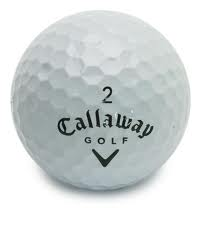
\includegraphics[width=.14\textwidth,trim=0mm 1cm 0mm 0cm,clip]{images/Callaway2}
\quad 
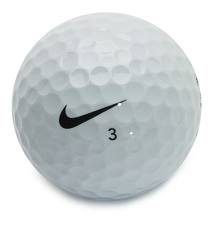
\includegraphics[width=.14\textwidth,trim=0mm 6mm 0mm 0mm,clip]{images/Nike3}
\quad 
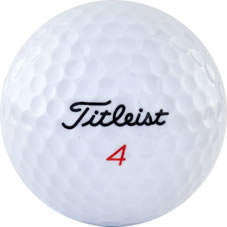
\includegraphics[width=.14\textwidth]{images/Titleist4}
\quad 

\includegraphics[width=.14\textwidth]{images/Noodle0}
\end{center}

Of the first 500 golf balls, 14 had either no number or a number other than 1, 2, 3, or 4.
The remaining 486 golf balls form our sample:


\begin{center}
\begin{tabular}{|c|c|c|c|c|}
\hline
1 & 2 & 3 & 4 & other\\
\hline
\hline
137 & 138 & 107 & 104 & 14 \\
\hline
\end{tabular}
\end{center}
We can enter this data into \R\ using the \function{c()} function.
\begin{knitrout}
\definecolor{shadecolor}{rgb}{.97, .97, .97}{\color{fgcolor}\begin{kframe}
\begin{flushleft}
\ttfamily\noindent
\hlsymbol{golfballs}{\ }\hlassignement{\usebox{\hlnormalsizeboxlessthan}-}{\ }\hlfunctioncall{c}\hlkeyword{(}\hlnumber{137}\hlkeyword{,}{\ }\hlnumber{138}\hlkeyword{,}{\ }\hlnumber{107}\hlkeyword{,}{\ }\hlnumber{104}\hlkeyword{)}\mbox{}
\normalfont
\end{flushleft}
\end{kframe}}
\end{knitrout}


\subsubsection{Coming up with a test statistic}
At this point, ask students what they think the data indicates about the hypothesis
that the four numbers are equally likely.  Students usually notice right away that 
there are a lot of 2's.  
%Looks like we have a lot of 1's and 2's and not so many 3's and 4's.  
But perhaps that's just the result of random sampling.  
We can generate random samples and see how the random samples compare with the actual data:
\begin{knitrout}
\definecolor{shadecolor}{rgb}{.97, .97, .97}{\color{fgcolor}\begin{kframe}
\begin{flushleft}
\ttfamily\noindent
\hlfunctioncall{table}\hlkeyword{(}\hlfunctioncall{rdata}\hlkeyword{(}\hlnumber{486}\hlkeyword{,}{\ }\hlnumber{1}\hlkeyword{:}\hlnumber{4}\hlkeyword{)}\hlkeyword{)}{\ }{\ }\hlcomment{\usebox{\hlnormalsizeboxhash}{\ }486{\ }draws{\ }from{\ }the{\ }numbers{\ }1{\ }thru{\ }4{\ }(equally{\ }likely)}\mbox{}
\normalfont
\end{flushleft}
\begin{verbatim}

  1   2   3   4 
128 125 111 122 
\end{verbatim}
\end{kframe}}
\end{knitrout}


\InstructorNote{\texttt{rgolfballs} can be generated
in advance if you don't want to distract your students
with thinking about how do create it.  There is a pre-built
\texttt{rgolfballs} in the \pkg{fastR} package.}%
It is useful to generate some more of these samples to get a better feel for the 
sampling distribution under the null:
\begin{knitrout}
\definecolor{shadecolor}{rgb}{.97, .97, .97}{\color{fgcolor}\begin{kframe}
\begin{flushleft}
\ttfamily\noindent
\hlfunctioncall{do}\hlkeyword{(}\hlnumber{25}\hlkeyword{)}{\ }\hlkeyword{*}{\ }\hlfunctioncall{table}\hlkeyword{(}\hlfunctioncall{rdata}\hlkeyword{(}\hlnumber{486}\hlkeyword{,}{\ }\hlnumber{1}\hlkeyword{:}\hlnumber{4}\hlkeyword{)}\hlkeyword{)}\mbox{}
\normalfont
\end{flushleft}
\end{kframe}}
\end{knitrout}

\begin{multicols}{3}
\begin{knitrout}
\definecolor{shadecolor}{rgb}{.97, .97, .97}{\color{fgcolor}\begin{kframe}
\begin{verbatim}
     1   2   3   4
1  122 126 112 126
2  118 128 131 109
3  128 112 143 103
4  119 133 120 114
5  115 128 118 125
6  107 136 118 125
7  128 111 117 130
8  122 117 117 130
9  111 132 116 127
10 127 119 113 127
11 124 127 102 133
12 137 128 112 109
13 106 136 107 137
14 126 129 109 122
15 139 127 103 117
16 111 136 115 124
17 140 108 124 114
18 129 114 119 124
19 121 108 120 137
20 128 114 121 123
21 127 114 121 124
22 129 119 131 107
23 125 127 133 101
24 120 123 126 117
25 145 127 105 109
\end{verbatim}
\end{kframe}}
\end{knitrout}

\end{multicols}

\FoodForThought[\centerline{Tip}]{
Have your students calculate test statistics mentally from
a small portion of the sampling distribution.  Assign each student a row or two,
then ask for a show of hands to see how many exceed the test statistic
calculated from the data.}%

From this we see that it is not incredibly unlikely to see a count of 138 or more.
(See samples \texttt{3, 15, 17, 25}.)
Students are often surprised just how often this occurs.

Once students understand the idea of a test statistic and how it is computed from data,
it's time to let the computer automate things.
First, we generate a better approximation to the sampling distribution assuming each number 
is equally likely.
\begin{knitrout}
\definecolor{shadecolor}{rgb}{.97, .97, .97}{\color{fgcolor}\begin{kframe}
\begin{flushleft}
\ttfamily\noindent
\hlsymbol{rgolfballs}{\ }\hlassignement{\usebox{\hlnormalsizeboxlessthan}-}{\ }\hlfunctioncall{do}\hlkeyword{(}\hlnumber{2000}\hlkeyword{)}{\ }\hlkeyword{*}{\ }\hlfunctioncall{table}\hlkeyword{(}\hlfunctioncall{rdata}\hlkeyword{(}\hlnumber{486}\hlkeyword{,}{\ }\hlnumber{1}\hlkeyword{:}\hlnumber{4}\hlkeyword{)}\hlkeyword{)}\mbox{}
\normalfont
\end{flushleft}
\end{kframe}}
\end{knitrout}

The \function{statTally()} function can tabulate and display the sampling distribution
and compared to the test statistic.
\begin{center}
\begin{knitrout}
\definecolor{shadecolor}{rgb}{.97, .97, .97}{\color{fgcolor}\begin{kframe}
\begin{flushleft}
\ttfamily\noindent
\hlfunctioncall{print}\hlkeyword{(}\hlfunctioncall{statTally}\hlkeyword{(}\hlsymbol{golfballs}\hlkeyword{,}{\ }\hlsymbol{rgolfballs}\hlkeyword{,}{\ }\hlsymbol{max}\hlkeyword{)}\hlkeyword{)}\mbox{}
\normalfont
\end{flushleft}
\begin{verbatim}
Test Stat function: max


Test Stat applied to sample data = 138

Test Stat applied to random data:

50% 90% 95% 99% 
132 141 143 149 
\end{verbatim}
\begin{verbatim}

Of the random samples
	 1622 ( 81.1 % ) had test stats < 138
	 62 ( 3.1 % ) had test stats = 138
	 316 ( 15.8 % ) had test stats > 138
\end{verbatim}
\begin{flushleft}
\ttfamily\noindent
\hlfunctioncall{ladd}\hlkeyword{(}\hlfunctioncall{print}\hlkeyword{(}\hlfunctioncall{panel.abline}\hlkeyword{(}\hlargument{v}{\ }\hlargument{=}{\ }\hlnumber{138}\hlkeyword{)}\hlkeyword{)}\hlkeyword{)}{\ }{\ }\hlcomment{\usebox{\hlnormalsizeboxhash}{\ }add{\ }a{\ }vertical{\ }line}\mbox{}
\normalfont
\end{flushleft}
\begin{verbatim}
NULL
\end{verbatim}


\centering{}\includegraphics{figures/fig-golfballs-max1} \includegraphics{figures/fig-golfballs-max2} 

\end{kframe}}
\end{knitrout}

\end{center}

\subsubsection{More test statistics}
One of the goals of this activity is to have the students understand the role of a test 
statistic.  Students are encouraged to dream up test statistics of their own.  The 
minimum count is often suggested as an alternative, so we try that one next.

\begin{knitrout}
\definecolor{shadecolor}{rgb}{.97, .97, .97}{\color{fgcolor}\begin{kframe}
\begin{flushleft}
\ttfamily\noindent
\hlfunctioncall{print}\hlkeyword{(}\hlfunctioncall{statTally}\hlkeyword{(}\hlsymbol{golfballs}\hlkeyword{,}{\ }\hlsymbol{rgolfballs}\hlkeyword{,}{\ }\hlsymbol{min}\hlkeyword{)}\hlkeyword{)}{\ }{\ }\hlcomment{\usebox{\hlnormalsizeboxhash}{\ }output{\ }surpressed.}\mbox{}
\normalfont
\end{flushleft}
\end{kframe}}
\end{knitrout}


These two test statistics (maximum count and minimum count) feel like they aren't 
making full use of our data.  
Perhaps we would do better if we looked at the difference between the maximum and 
minimum counts.
This requires writing a simple function.
\FoodForThought{See Section~\ref{sec:writingFunctions} for a tutorial
on writing your own functions.}

\begin{center}
\begin{knitrout}
\definecolor{shadecolor}{rgb}{.97, .97, .97}{\color{fgcolor}\begin{kframe}
\begin{flushleft}
\ttfamily\noindent
\hlsymbol{mystat1}{\ }\hlassignement{\usebox{\hlnormalsizeboxlessthan}-}{\ }\hlkeyword{function}\hlkeyword{(}\hlformalargs{x}\hlkeyword{)}{\ }\hlkeyword{\usebox{\hlnormalsizeboxopenbrace}}\hspace*{\fill}\\
\hlstd{}{\ }{\ }{\ }{\ }\hlfunctioncall{diff}\hlkeyword{(}\hlfunctioncall{range}\hlkeyword{(}\hlsymbol{x}\hlkeyword{)}\hlkeyword{)}\hspace*{\fill}\\
\hlstd{}\hlkeyword{\usebox{\hlnormalsizeboxclosebrace}}\hspace*{\fill}\\
\hlstd{}\hlfunctioncall{print}\hlkeyword{(}\hlfunctioncall{statTally}\hlkeyword{(}\hlsymbol{golfballs}\hlkeyword{,}{\ }\hlsymbol{rgolfballs}\hlkeyword{,}{\ }\hlsymbol{mystat1}\hlkeyword{,}{\ }\hlargument{v}{\ }\hlargument{=}{\ }\hlfunctioncall{mystat1}\hlkeyword{(}\hlsymbol{golfballs}\hlkeyword{)}\hlkeyword{)}\hlkeyword{)}{\ }{\ }\hlcomment{\usebox{\hlnormalsizeboxhash}{\ }add{\ }a{\ }vertical{\ }line}\mbox{}
\normalfont
\end{flushleft}
\begin{verbatim}
Test Stat function: mystat1


Test Stat applied to sample data = 34

Test Stat applied to random data:

  50%   90%   95%   99% 
22.00 36.00 40.00 49.01 
\end{verbatim}
\begin{verbatim}

Of the random samples
	 1712 ( 85.6 % ) had test stats < 34
	 42 ( 2.1 % ) had test stats = 34
	 246 ( 12.3 % ) had test stats > 34
\end{verbatim}


\centering{}\includegraphics{figures/fig-golfballs-range1} \includegraphics{figures/fig-golfballs-range2} 

\end{kframe}}
\end{knitrout}

\end{center}

\subsubsection{The World's Worst Test Statistic}

Usually I get lucky and someone will suggest the world's worst test statistic:
The sum of the differences between the counts and $486/4 = 121.5$.
\begin{center}
\begin{knitrout}
\definecolor{shadecolor}{rgb}{.97, .97, .97}{\color{fgcolor}\begin{kframe}
\begin{flushleft}
\ttfamily\noindent
\hlsymbol{mystat2}{\ }\hlassignement{\usebox{\hlnormalsizeboxlessthan}-}{\ }\hlkeyword{function}\hlkeyword{(}\hlformalargs{x}\hlkeyword{)}{\ }\hlkeyword{\usebox{\hlnormalsizeboxopenbrace}}\hspace*{\fill}\\
\hlstd{}{\ }{\ }{\ }{\ }\hlfunctioncall{sum}\hlkeyword{(}\hlsymbol{x}{\ }\hlkeyword{-}{\ }\hlnumber{121.5}\hlkeyword{)}\hspace*{\fill}\\
\hlstd{}\hlkeyword{\usebox{\hlnormalsizeboxclosebrace}}\hspace*{\fill}\\
\hlstd{}\hlfunctioncall{print}\hlkeyword{(}\hlfunctioncall{statTally}\hlkeyword{(}\hlsymbol{golfballs}\hlkeyword{,}{\ }\hlsymbol{rgolfballs}\hlkeyword{,}{\ }\hlsymbol{mystat2}\hlkeyword{)}\hlkeyword{)}\mbox{}
\normalfont
\end{flushleft}
\begin{verbatim}
Test Stat function: mystat2


Test Stat applied to sample data = 0

Test Stat applied to random data:

50% 90% 95% 99% 
  0   0   0   0 
\end{verbatim}
\begin{verbatim}

Of the random samples
	 0 ( 0 % ) had test stats < 0
	 2000 ( 100 % ) had test stats = 0
	 0 ( 0 % ) had test stats > 0
\end{verbatim}


\centering{}\includegraphics{figures/fig-golfballs-worst1} \includegraphics{figures/fig-golfballs-worst2} 

\end{kframe}}
\end{knitrout}

\end{center}
This test statistic is bad because it doesn't depend on the data, so 
the distribution of the test statistic is the same whether the null hypothesis 
is true or false.

\InstructorNote[\centerline{Tip}]{As students come up with test statistics, let them
name them, or name them after them (S for the Smith statistic, etc.)
It adds to the fun of the activity and mirrors how the statistics they will
learn about got their names.}%
But it is close to a good idea.  Let's add in an absolute value\dots
\begin{center}
\begin{knitrout}
\definecolor{shadecolor}{rgb}{.97, .97, .97}{\color{fgcolor}\begin{kframe}
\begin{flushleft}
\ttfamily\noindent
\hlsymbol{sad}{\ }\hlassignement{\usebox{\hlnormalsizeboxlessthan}-}{\ }\hlkeyword{function}\hlkeyword{(}\hlformalargs{x}\hlkeyword{)}{\ }\hlkeyword{\usebox{\hlnormalsizeboxopenbrace}}\hspace*{\fill}\\
\hlstd{}{\ }{\ }{\ }{\ }\hlfunctioncall{sum}\hlkeyword{(}\hlfunctioncall{abs}\hlkeyword{(}\hlsymbol{x}{\ }\hlkeyword{-}{\ }\hlnumber{121.5}\hlkeyword{)}\hlkeyword{)}\hspace*{\fill}\\
\hlstd{}\hlkeyword{\usebox{\hlnormalsizeboxclosebrace}}\hspace*{\fill}\\
\hlstd{}\hlfunctioncall{print}\hlkeyword{(}\hlfunctioncall{statTally}\hlkeyword{(}\hlsymbol{golfballs}\hlkeyword{,}{\ }\hlsymbol{rgolfballs}\hlkeyword{,}{\ }\hlsymbol{sad}\hlkeyword{,}{\ }\hlargument{v}{\ }\hlargument{=}{\ }\hlfunctioncall{sad}\hlkeyword{(}\hlsymbol{golfballs}\hlkeyword{)}\hlkeyword{)}\hlkeyword{)}\mbox{}
\normalfont
\end{flushleft}
\begin{verbatim}
Test Stat function: sad


Test Stat applied to sample data = 64

Test Stat applied to random data:

  50%   90%   95%   99% 
30.00 48.00 54.00 67.01 
\end{verbatim}
\begin{verbatim}

Of the random samples
	 1970 ( 98.5 % ) had test stats < 64
	 5 ( 0.25 % ) had test stats = 64
	 25 ( 1.25 % ) had test stats > 64
\end{verbatim}


\centering{}\includegraphics{figures/fig-golfballs-var1} \includegraphics{figures/fig-golfballs-var2} 

\end{kframe}}
\end{knitrout}

\end{center}
\InstructorNote{It is a matter of teaching style whether you write this 
function with the magic number 121.5 hard-coded in or use
\code{mean(x)} instead.  The latter is preferable for generalizable 
method, of course.  But the former may have pedagogical advantages, 
especially in the Intro Stats course.}%

Squaring those differences (or equivalently using the standard deviation or variance)
is also often suggested.

\begin{center}
\begin{knitrout}
\definecolor{shadecolor}{rgb}{.97, .97, .97}{\color{fgcolor}\begin{kframe}
\begin{flushleft}
\ttfamily\noindent
\hlfunctioncall{print}\hlkeyword{(}\hlfunctioncall{statTally}\hlkeyword{(}\hlsymbol{golfballs}\hlkeyword{,}{\ }\hlsymbol{rgolfballs}\hlkeyword{,}{\ }\hlsymbol{var}\hlkeyword{,}{\ }\hlargument{v}{\ }\hlargument{=}{\ }\hlfunctioncall{var}\hlkeyword{(}\hlsymbol{golfballs}\hlkeyword{)}\hlkeyword{)}\hlkeyword{)}\mbox{}
\normalfont
\end{flushleft}
\begin{verbatim}
Test Stat function: var


Test Stat applied to sample data = 343

Test Stat applied to random data:

   50%    90%    95%    99% 
 97.67 251.87 313.67 481.13 
\end{verbatim}
\begin{verbatim}

Of the random samples
	 1925 ( 96.25 % ) had test stats < 343
	 1 ( 0.05 % ) had test stats = 343
	 74 ( 3.7 % ) had test stats > 343
\end{verbatim}


\centering{}\includegraphics{figures/fig-golfballs-var1} \includegraphics{figures/fig-golfballs-var2} 

\end{kframe}}
\end{knitrout}

\end{center}

This example illustrates some important ideas about hypothesis testing, namely.
\authNote{Need to decide where the planets analogy goes relative to this.}%

\begin{boxedText}
\begin{enumerate}
\item The test statistic must summarize the evidence we will use to 
judge the null hypothesis \emph{in a single number} computed from our sample.
\item
We judge the test statistic computed from our sample by comparing it to
test statistics computed on random samples \emph{assuming the Null Hypothesis is true.}
\item
Some test statistics work better than others.

A good test statistic should look quite different when the null hypothesis 
is true from how it looks when the null hypothesis is false.  
(This is a first hint at the idea of power.)
\end{enumerate}
\end{boxedText}

\section{The Multi-World Metaphor for Statistical Inference}

\begin{comment}
In this section we move toward a more systematic approach to 
empirical methods with goal of providing a flexible tool 
that works in a wide range of situations.
\end{comment}

Statistical inference is hard to teach.%
\footnote{Here we are considering only the
  frequentist version of inference.  The Bayesian approach is
  different and has different features that make it hard to teach and
  understand.  In these notes, we will be agnostic about frequentist
  vs Bayesian, except to acknowledge that, for good or bad, the
  frequentist approach is vastly dominant in introductory statistics courses.}
Often, instead of teaching
the logic of inference, we teach methods and techniques for
calculating the quantities used in inference: standard errors,
t-statistics, p-values, etc.  

Perhaps because students don't understand the logic, they have strong
misconceptions about confidence intervals and, especially, about
p-values.  For example, even among professional scientists, the
mainstream (mis)-understanding of p-values is that they reflect the
probability that the null hypothesis is correct.

Part of the reason why statistical inference is hard to grasp is that
the logic is genuinely hard.  It involves contrapositives, it
involves conditional probabilities, it involves ``hypotheses.''
And what is a hypothesis?  To a scientist, it is a kind of theory, an idea of how
things work, an idea to be proven through lab or field research or the
collection of data.  
\FoodForThought{The simpler ``definition'' is a useful way to describe this to students, but
it is not equivalent to the dictionary definition which includes an important notion
of the reason for hypotheses.  
A hypothesis is a statement that is posed 
for the purposes of determining what would follow if the statement were true.  This is 
the sense of `hypothesis of a theorem'.  It is also the sense of the null hypothesis.
We assume the null hypothesis is true and `see what follows' from that assumption.
Unfortunately, it is not the way this word is often used in high school science courses.}%
But statistics hews not to the scientist's but to
the philosopher's or logician's rather abstract notion 
of a hypothesis: a ``proposition made as a basis for reasoning, without any
assumption of its truth.''  (Oxford American Dictionaries)  Or more simply:

\begin{center}
A hypothesis is a statement that may be true or false.
\end{center}

What kind of scientist would frame a hypothesis without some disposition to
think it might be true?  Only a philosopher or a logician.
\FoodForThought{Thought of another way, the scientists have conflated 
the words 'hypothesis' and 'conjecture'.
}%

To help connect the philosophy and logic of statistical hypotheses
with the sensibilities of scientists, 
it might be helpful to draw from the theory of kinesthetic learning
--- an active theory, not a philosophical proposition --- that learning is enhanced by
carrying out a physical activity.
Many practitioners of the reform style of teaching statistics engage
in the kinesthetic style; they have students draw M\&Ms from a bag
and count the brown ones, they have students walk randomly to see how
far they get after $n$ steps \cite{kaplan-2009-book}, or they toss a globe around the classroom
to see how often a students' index finger lands in the ocean \cite{gelm:nola:2002}.

To teach hypothesis testing in a kinesthetic way, you need a physical
representation of the various hypotheses found in statistical
inference.  One way to do this involves not the actual physical
activity of truly kinesthetic learning, but concrete stories of making
different sorts of trips to different sorts of worlds.  
A hypothesis may be true on some worlds and false on others.
On some planets we will know whether a hypothesis is true or false,
on others, the truth of a hypothesis is an open question.
%To that end, we humbly offer physical analogs of the various hypotheses: the planets.

Of course, the planet that we care about, the place about which we
want to be able to draw conclusions.  It's Planet Earth:

\centerline{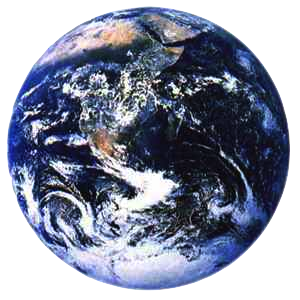
\includegraphics[width=1.2in]{images/planet_earth.png}}

We want to know which hypotheses are true on Earth and which are false.
%This is not a hypothesis; it's reality.  
But Earth is a big place and complicated,
and it's hard to know exactly what's going on.  So, to
deal with the limits of our abilities to collect data and to
understand complexity, statistical inference involves a different set
of planets.  These planets resemble Planet Earth in some ways and not in others.  
But they are simple enough that we know exactly what's happening on them, 
so we know which hypotheses are true and which are false on these planets.
%they are ``proposition[s] made as a
%basis for reasoning, without any assumption of [their] truth.''  \cite{needCitation}

These planets are:

\begin{center}
\begin{tabular}{ccc}
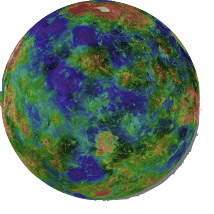
\includegraphics[width=0.6in]{images/planet-sample.png} &
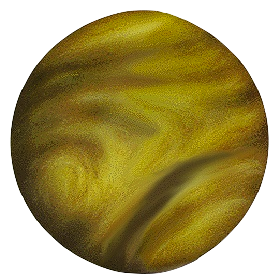
\includegraphics[width=1.2in]{images/venus.png} &

\includegraphics[width=1.4in]{images/planet-alt.png} \\
Planet Sample & Planet Null & Planet Alt\\
\end{tabular}
\end{center}

Planet Sample is populated entirely with the cases we have collected
on Planet Earth.  As such, it somewhat resembles Earth, but many of
the details are missing, perhaps even whole countries or continents or seas.
And of course, it is much smaller than Planet Earth.

Planet Null is a boring planet.  Nothing is happening there. Express
it how you will: All groups all have the same mean values.
The model coefficients are zero. Different variables are unrelated to
one another.  Dullsville.  But even if it's dull, it's not a polished
billiard ball that looks the same from every perspective.  It's the
clay from which Adam was created, the ashes and dust to which man
returns.  But it varies from place to place, and that variation is not
informative. It's just random.

Finally, there is Planet Alt.  This is a cartoon planet, a caricature,
a simplified representation of our idea of what is (or might be) going on, 
our theory of how the world might be working.  It's not going to be exactly the
same as Planet Earth.  For one thing, our theory might be wrong.  But
also, no theory is going to capture all the detail and complexity of
the real world.

In teaching statistical inference in a pseudo-kinesthetic way, we use
the computer to let students construct each of the planets.  
Then, working on that planet, the student can
carry out simulations of familiar statistical operations.   Those
simulations tell the student what they are likely to see \emph{if they were on that planet}.   
Our goal is to figure out whether Earth looks more like Planet Null or more like 
Planet Alt.
\authNote{rjp: Are we OK with this last sentence?  Perhaps it will get us into trouble, but I'll
leave it for now and see how it goes.}

For the professional statisticians, the planet metaphor is
unnecessary.  The professional has learned to keep straight the
various roles of the null and alternative hypothesis, and why one uses
a sample standard error to estimate the standard deviation of the
sampling distribution from the population.  But most students find the
array of concepts confusing and make basic categorical errors.  The
concrete nature of the planets simplifies the task of keeping the
concepts in order.  For instance, Type I errors only occur 
on Planet Null.  You have to be on Planet Alt to make a Type II
error.  And, of course, no matter how many (re)samples we make on
Planet Sample, it's never going to look more like Earth than the
sample itself.

\subsection{The Sampling Distribution}

Section \ref{sec:taking-randomness-seriously} shows some examples of
drawing random samples repeatedly from a set of data.  To discuss the
sampling distribution, it's helpful to make clear that the sampling
distribution refers to results from the \textbf{population}.  In the planet
metaphor, this means that the samples are drawn from Planet Earth:

\centerline{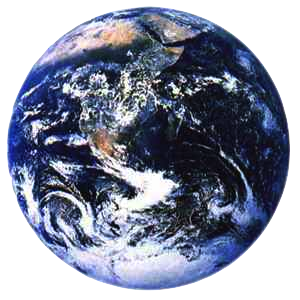
\includegraphics[width=1.2in]{images/planet_earth.png}}

It can be a challenge to find a compelling example where you have the
population, rather than a sample, in hand.  Sports statistics provide
one plausible setting, where
you have, for example, the names and attributes of every professional
player.  The ability to sample from Earth mapping software
provides another compelling setting.  (See Section~\ref{sec:googleMap}.)
\authNote{We don't really have the whole population here either.  I guess perhaps
Google does.  But we only get to sample from their data base.}%

For our example, we will take the complete list of results from a
running race held in Washington, D.C. in April 2005 --- the Cherry
Blossom Ten-Mile Run.  
The data set gives the \VN{sex}, \VN{age}, and \VN{net} running time
(start line to finish line) for each of the 8636 runners who
participated: the population of runners in that race.

\authNoted{I changed \verb!our.population! to \verb!population!.  If you really like the old
name, you can change it back.  --rjp --- Yours is better. DTK  Thanks
for adding TenMileRace to the package.}
\begin{knitrout}
\definecolor{shadecolor}{rgb}{.97, .97, .97}{\color{fgcolor}\begin{kframe}
\begin{flushleft}
\ttfamily\noindent
\hlsymbol{population}{\ }\hlassignement{\usebox{\hlnormalsizeboxlessthan}-}{\ }\hlsymbol{TenMileRace}\hspace*{\fill}\\
\hlstd{}\hlfunctioncall{nrow}\hlkeyword{(}\hlsymbol{population}\hlkeyword{)}\mbox{}
\normalfont
\end{flushleft}
\begin{verbatim}
[1] 8636
\end{verbatim}
\end{kframe}}
\end{knitrout}


If you have the population on the computer, there's little point
in taking a random sample.  But the point here is to illustrate the
consequences of taking a sample.  So, imagine that in fact it was
difficult or expensive or dangerous or destructive to collect the data on a runner,
so you want to examine just a small subset of the population.

Let's collect a sample of 100 runners:
\begin{knitrout}
\definecolor{shadecolor}{rgb}{.97, .97, .97}{\color{fgcolor}\begin{kframe}
\begin{flushleft}
\ttfamily\noindent
\hlsymbol{planet.sample}{\ }\hlassignement{\usebox{\hlnormalsizeboxlessthan}-}{\ }\hlfunctioncall{sample}\hlkeyword{(}\hlsymbol{population}\hlkeyword{,}{\ }\hlnumber{100}\hlkeyword{)}\mbox{}
\normalfont
\end{flushleft}
\end{kframe}}
\end{knitrout}


With that sample, we can calculate whatever statistics are of
interest to us, for instance:
\begin{knitrout}
\definecolor{shadecolor}{rgb}{.97, .97, .97}{\color{fgcolor}\begin{kframe}
\begin{flushleft}
\ttfamily\noindent
\hlfunctioncall{with}\hlkeyword{(}\hlsymbol{planet.sample}\hlkeyword{,}{\ }\hlfunctioncall{mean}\hlkeyword{(}\hlsymbol{age}\hlkeyword{)}\hlkeyword{)}\mbox{}
\normalfont
\end{flushleft}
\begin{verbatim}
 mean 
36.84 
\end{verbatim}
\begin{flushleft}
\ttfamily\noindent
\hlfunctioncall{with}\hlkeyword{(}\hlsymbol{planet.sample}\hlkeyword{,}{\ }\hlfunctioncall{sd}\hlkeyword{(}\hlsymbol{age}\hlkeyword{)}\hlkeyword{)}\mbox{}
\normalfont
\end{flushleft}
\begin{verbatim}
   sd 
10.34 
\end{verbatim}
\begin{flushleft}
\ttfamily\noindent
\hlfunctioncall{with}\hlkeyword{(}\hlsymbol{planet.sample}\hlkeyword{,}{\ }\hlfunctioncall{mean}\hlkeyword{(}\hlsymbol{sex}{\ }=={\ }\hlstring{"{}F"{}}\hlkeyword{)}\hlkeyword{)}\mbox{}
\normalfont
\end{flushleft}
\begin{verbatim}
mean 
0.47 
\end{verbatim}
\begin{flushleft}
\ttfamily\noindent
\hlfunctioncall{lm}\hlkeyword{(}\hlsymbol{net}{\ }\hlkeyword{\urltilda{}}{\ }\hlsymbol{age}{\ }\hlkeyword{+}{\ }\hlsymbol{sex}\hlkeyword{,}{\ }\hlargument{data}{\ }\hlargument{=}{\ }\hlsymbol{planet.sample}\hlkeyword{)}\mbox{}
\normalfont
\end{flushleft}
\begin{verbatim}

Call:
lm(formula = net ~ age + sex, data = planet.sample)

Coefficients:
(Intercept)          age         sexM  
       5554           14         -957  

\end{verbatim}
\end{kframe}}
\end{knitrout}


These various numbers are informative in their own way about the
sample, but it's important to know how they might relate to the
population.  For example, how precise are these numbers?  That is, if
someone had collected a different random sample, how different would
their results likely be?

Given that we have the population in hand, that we're on Planet Earth,
we can go back and collect such samples many more times and study how much
they vary one to the other.  We'll do this by replacing
\variable{planet.sample} with a command to sample anew from the population.

\begin{knitrout}
\definecolor{shadecolor}{rgb}{.97, .97, .97}{\color{fgcolor}\begin{kframe}
\begin{flushleft}
\ttfamily\noindent
\hlfunctioncall{with}\hlkeyword{(}\hlfunctioncall{sample}\hlkeyword{(}\hlsymbol{population}\hlkeyword{,}{\ }\hlnumber{100}\hlkeyword{)}\hlkeyword{,}{\ }\hlfunctioncall{mean}\hlkeyword{(}\hlsymbol{age}\hlkeyword{)}\hlkeyword{)}\mbox{}
\normalfont
\end{flushleft}
\begin{verbatim}
 mean 
36.92 
\end{verbatim}
\begin{flushleft}
\ttfamily\noindent
\hlfunctioncall{with}\hlkeyword{(}\hlfunctioncall{sample}\hlkeyword{(}\hlsymbol{population}\hlkeyword{,}{\ }\hlnumber{100}\hlkeyword{)}\hlkeyword{,}{\ }\hlfunctioncall{sd}\hlkeyword{(}\hlsymbol{age}\hlkeyword{)}\hlkeyword{)}\mbox{}
\normalfont
\end{flushleft}
\begin{verbatim}
   sd 
10.95 
\end{verbatim}
\begin{flushleft}
\ttfamily\noindent
\hlfunctioncall{with}\hlkeyword{(}\hlfunctioncall{sample}\hlkeyword{(}\hlsymbol{population}\hlkeyword{,}{\ }\hlnumber{100}\hlkeyword{)}\hlkeyword{,}{\ }\hlfunctioncall{mean}\hlkeyword{(}\hlsymbol{sex}{\ }=={\ }\hlstring{"{}F"{}}\hlkeyword{)}\hlkeyword{)}\mbox{}
\normalfont
\end{flushleft}
\begin{verbatim}
mean 
0.56 
\end{verbatim}
\begin{flushleft}
\ttfamily\noindent
\hlfunctioncall{lm}\hlkeyword{(}\hlsymbol{net}{\ }\hlkeyword{\urltilda{}}{\ }\hlsymbol{age}{\ }\hlkeyword{+}{\ }\hlsymbol{sex}\hlkeyword{,}{\ }\hlargument{data}{\ }\hlargument{=}{\ }\hlfunctioncall{sample}\hlkeyword{(}\hlsymbol{population}\hlkeyword{,}{\ }\hlnumber{100}\hlkeyword{)}\hlkeyword{)}\mbox{}
\normalfont
\end{flushleft}
\begin{verbatim}

Call:
lm(formula = net ~ age + sex, data = sample(population, 100))

Coefficients:
(Intercept)          age         sexM  
     5403.0         15.4       -854.0  

\end{verbatim}
\end{kframe}}
\end{knitrout}


Slightly different results!  To quantify this, repeat the sampling
process many times and look at the distribution: the \term{sampling distribution}.

\begin{knitrout}
\definecolor{shadecolor}{rgb}{.97, .97, .97}{\color{fgcolor}\begin{kframe}
\begin{flushleft}
\ttfamily\noindent
\hlsymbol{sample.means}{\ }\hlassignement{\usebox{\hlnormalsizeboxlessthan}-}{\ }\hlfunctioncall{do}\hlkeyword{(}\hlnumber{500}\hlkeyword{)}{\ }\hlkeyword{*}{\ }\hlfunctioncall{with}\hlkeyword{(}\hlfunctioncall{sample}\hlkeyword{(}\hlsymbol{population}\hlkeyword{,}{\ }\hlnumber{100}\hlkeyword{)}\hlkeyword{,}{\ }\hlfunctioncall{mean}\hlkeyword{(}\hlsymbol{age}\hlkeyword{)}\hlkeyword{)}\hspace*{\fill}\\
\hlstd{}\hlsymbol{sample.sds}{\ }\hlassignement{\usebox{\hlnormalsizeboxlessthan}-}{\ }\hlfunctioncall{do}\hlkeyword{(}\hlnumber{500}\hlkeyword{)}{\ }\hlkeyword{*}{\ }\hlfunctioncall{with}\hlkeyword{(}\hlfunctioncall{sample}\hlkeyword{(}\hlsymbol{population}\hlkeyword{,}{\ }\hlnumber{100}\hlkeyword{)}\hlkeyword{,}{\ }\hlfunctioncall{sd}\hlkeyword{(}\hlsymbol{age}\hlkeyword{)}\hlkeyword{)}\hspace*{\fill}\\
\hlstd{}\hlsymbol{sample.props}{\ }\hlassignement{\usebox{\hlnormalsizeboxlessthan}-}{\ }\hlfunctioncall{do}\hlkeyword{(}\hlnumber{500}\hlkeyword{)}{\ }\hlkeyword{*}{\ }\hlfunctioncall{with}\hlkeyword{(}\hlfunctioncall{sample}\hlkeyword{(}\hlsymbol{population}\hlkeyword{,}{\ }\hlnumber{100}\hlkeyword{)}\hlkeyword{,}{\ }\hlfunctioncall{mean}\hlkeyword{(}\hlsymbol{sex}{\ }==\hspace*{\fill}\\
\hlstd{}{\ }{\ }{\ }{\ }\hlstring{"{}F"{}}\hlkeyword{)}\hlkeyword{)}\hspace*{\fill}\\
\hlstd{}\hlsymbol{sample.regressions}{\ }\hlassignement{\usebox{\hlnormalsizeboxlessthan}-}{\ }\hlfunctioncall{do}\hlkeyword{(}\hlnumber{500}\hlkeyword{)}{\ }\hlkeyword{*}{\ }\hlfunctioncall{lm}\hlkeyword{(}\hlsymbol{net}{\ }\hlkeyword{\urltilda{}}{\ }\hlsymbol{age}{\ }\hlkeyword{+}{\ }\hlsymbol{sex}\hlkeyword{,}{\ }\hlargument{data}{\ }\hlargument{=}{\ }\hlfunctioncall{sample}\hlkeyword{(}\hlsymbol{population}\hlkeyword{,}\hspace*{\fill}\\
\hlstd{}{\ }{\ }{\ }{\ }\hlnumber{100}\hlkeyword{)}\hlkeyword{)}\mbox{}
\normalfont
\end{flushleft}
\end{kframe}}
\end{knitrout}


You can display the sampling distribution in several ways: histograms,
box-and-whisker plots, density plots.  This is worth doing with the
class.  Make sure to point out that the distribution depends on the
statistic being calculated: in the above examples, the mean age, the standard deviation of
ages, the fraction of runners who are female, the relationship between
running time and \VN{sex} and \VN{age}.  (We'll get to the dependence
on sample size in a little bit.)

Insofar as we want to be able to characterize the repeatability of the
results of the sampling process, it's worth describing it in terms of the spread of
the distribution: for instance, the standard deviation.  Of course, when talking
about a sampling distribution, we give another name to the standard
deviation: the {\em standard error}.   Actually calculating the
standard error may perhaps solidify in the students mind that it is a
standard deviation.

\begin{knitrout}
\definecolor{shadecolor}{rgb}{.97, .97, .97}{\color{fgcolor}\begin{kframe}
\begin{flushleft}
\ttfamily\noindent
\hlfunctioncall{sd}\hlkeyword{(}\hlsymbol{sample.means}\hlkeyword{)}{\ }{\ }\hlcomment{\usebox{\hlnormalsizeboxhash}{\ }standard{\ }error{\ }for{\ }mean{\ }age}\mbox{}
\normalfont
\end{flushleft}
\begin{verbatim}
 mean 
1.016 
\end{verbatim}
\begin{flushleft}
\ttfamily\noindent
\hlfunctioncall{sd}\hlkeyword{(}\hlsymbol{sample.sds}\hlkeyword{)}{\ }{\ }\hlcomment{\usebox{\hlnormalsizeboxhash}{\ }standard{\ }error{\ }for{\ }sd{\ }of{\ }age}\mbox{}
\normalfont
\end{flushleft}
\begin{verbatim}
    sd 
0.7808 
\end{verbatim}
\begin{flushleft}
\ttfamily\noindent
\hlfunctioncall{sd}\hlkeyword{(}\hlsymbol{sample.props}\hlkeyword{)}{\ }{\ }\hlcomment{\usebox{\hlnormalsizeboxhash}{\ }standard{\ }error{\ }for{\ }fraction{\ }female}\mbox{}
\normalfont
\end{flushleft}
\begin{verbatim}
   mean 
0.04895 
\end{verbatim}
\begin{flushleft}
\ttfamily\noindent
\hlfunctioncall{sd}\hlkeyword{(}\hlsymbol{sample.regressions}\hlkeyword{)}{\ }{\ }\hlcomment{\usebox{\hlnormalsizeboxhash}{\ }standard{\ }errors{\ }for{\ }regression{\ }statistics}\mbox{}
\normalfont
\end{flushleft}
\begin{verbatim}
Intercept       age      sexM     sigma r-squared 
344.97489   9.58257 191.30069  78.45032   0.06571 
\end{verbatim}
\end{kframe}}
\end{knitrout}



\begin{example}
This is an activity to carry out in class, with each student or pair
of students at a computer.

\begin{enumerate}
  \item Make sure you can replicate the calculations for the standard
    error of one of the statistics in the \dfn{TenMileRace} example with a
    sample of size $n=100$.  Your reproduction won't be exact, but it
    should be reasonably close.
  \item Now repeat the calculations, but use sample sizes that are
    larger.  From $n=100$, increase to $n=400$, then $n=1600$, then $n=6400$.
    How does the standard error depend on $n$?  Does larger $n$
    lead to a bigger or smaller standard error?  Which of these
    formulas most closely matches the pattern you see:
    \begin{enumerate}
      \item The standard error increases with $n$.
      \item The standard error increases with $\sqrt{n}$.
      \item The standard error gets smaller with increasing $n$ with
       the pattern $1/\sqrt{n}$.
      \item The standard error gets smaller with increasing $n$ with
       the pattern $1/n$.
   \end{enumerate}
    \item Use the pattern you observed to predict what will be the
      standard error for a sample of size $n=1000$.  Then carry out
      the actual simulation of repeated sampling using that sample size and compare your
      prediction to the result you actually got.
      
    \item In the above, you used \code{do(500)} replications of
      random sampling.  Suppose you use \code{do(100)} or
      \code{do(2000)} replications instead?  Do your results depend
      systematically on the number of replications?
 
 \end{enumerate}
\end{example}


\subsection{The Re-Sampling Distribution}

The sampling distribution is a lovely theoretical thing.  But if it
were easy to replicate taking a sample over and over again,
wouldn't you just take a larger sample in the first place?  The
practical problem you face is that the sample you took was collected
with difficulty and expense.  There's no way you are going to go back
and repeat the process that was so difficult in the first place.
Remember, real samples from the real population (on planet Earth) 
can't be obtained by simply asking a computer to sample for us.

This is where Planet Sample comes in.
\smallskip

\centerline{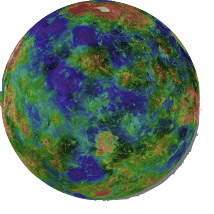
\includegraphics[width=0.6in]{images/planet-sample.png}}

\FoodForThought{In our example we have access to the entire population, but this 
is not typically the case.}%
Although Planet Earth is very large and we have only incomplete information about
it, all the data for Planet Sample is in our computer. So 

\begin{center}
\emph{Although sampling
from Planet Earth is difficult, sampling from Planet Sample is easy}.
\end{center}

\authNote{R' deleted: 
You create Planet Sample yourself.  You do this by taking your sample
using it to populate Planet Sample.  It consists of many, many copies of your sample.}

To illustrate, here's a sample from the running population:
\begin{knitrout}
\definecolor{shadecolor}{rgb}{.97, .97, .97}{\color{fgcolor}\begin{kframe}
\begin{flushleft}
\ttfamily\noindent
\hlsymbol{planet.sample}{\ }\hlassignement{=}{\ }\hlfunctioncall{sample}\hlkeyword{(}\hlsymbol{population}\hlkeyword{,}{\ }\hlnumber{100}\hlkeyword{)}{\ }{\ }\hlcomment{\usebox{\hlnormalsizeboxhash}{\ }one{\ }sample{\ }from{\ }the{\ }population}\mbox{}
\normalfont
\end{flushleft}
\end{kframe}}
\end{knitrout}

In reality, of course, you wouldn't run a command to create the sample.  
You would go out and do the hard work of randomly selecting cases from your population,
measuring their relevant attributes, and recording that data.  
So let's pretend that's what we did.  Pretend that 
\variable{planet.sample} is the result of laborious data collection.


Now you can go through the exact calculations you did to construct the
sampling distribution (on Planet Earth), but instead sample from 
Planet Sample:
\begin{knitrout}
\definecolor{shadecolor}{rgb}{.97, .97, .97}{\color{fgcolor}\begin{kframe}
\begin{flushleft}
\ttfamily\noindent
\hlfunctioncall{with}\hlkeyword{(}\hlfunctioncall{sample}\hlkeyword{(}\hlsymbol{planet.sample}\hlkeyword{,}{\ }\hlnumber{100}\hlkeyword{)}\hlkeyword{,}{\ }\hlfunctioncall{mean}\hlkeyword{(}\hlsymbol{age}\hlkeyword{)}\hlkeyword{)}\mbox{}
\normalfont
\end{flushleft}
\begin{verbatim}
 mean 
36.59 
\end{verbatim}
\begin{flushleft}
\ttfamily\noindent
\hlfunctioncall{with}\hlkeyword{(}\hlfunctioncall{sample}\hlkeyword{(}\hlsymbol{planet.sample}\hlkeyword{,}{\ }\hlnumber{100}\hlkeyword{)}\hlkeyword{,}{\ }\hlfunctioncall{mean}\hlkeyword{(}\hlsymbol{age}\hlkeyword{)}\hlkeyword{)}\mbox{}
\normalfont
\end{flushleft}
\begin{verbatim}
 mean 
36.59 
\end{verbatim}
\begin{flushleft}
\ttfamily\noindent
\hlfunctioncall{with}\hlkeyword{(}\hlfunctioncall{sample}\hlkeyword{(}\hlsymbol{planet.sample}\hlkeyword{,}{\ }\hlnumber{100}\hlkeyword{)}\hlkeyword{,}{\ }\hlfunctioncall{mean}\hlkeyword{(}\hlsymbol{age}\hlkeyword{)}\hlkeyword{)}\mbox{}
\normalfont
\end{flushleft}
\begin{verbatim}
 mean 
36.59 
\end{verbatim}
\end{kframe}}
\end{knitrout}




Wait, something went wrong.  We are getting the same mean every time.  The reason is that
Planet Sample is small.  It only has 100 inhabitants and we are sampling all 100 each time.
We could take smaller samples, but we want to learn about samples of the same size as 
our actual sample, so that's not a good option. 


Our solution to this problem is to sample \emph{with replacement}.  That is, we will select
an inhabitant of Planet Sample, record the appropriate data, and then put them back on the planet
-- possibly selecting that same inhabitant again later in our sample.  We'll call sampling with
replacement from Planet Sample \term{resampling} for short.  The \function{resample()} function
in the \pkg{mosaic} package can do this as easily as sampling without replacement.

\Caution{Remember to use \function{resample()} rather than 
\function{sample()} to compute a resampling distribution.}
\begin{knitrout}
\definecolor{shadecolor}{rgb}{.97, .97, .97}{\color{fgcolor}\begin{kframe}
\begin{flushleft}
\ttfamily\noindent
\hlfunctioncall{with}\hlkeyword{(}\hlfunctioncall{resample}\hlkeyword{(}\hlsymbol{planet.sample}\hlkeyword{,}{\ }\hlnumber{100}\hlkeyword{)}\hlkeyword{,}{\ }\hlfunctioncall{mean}\hlkeyword{(}\hlsymbol{age}\hlkeyword{)}\hlkeyword{)}\mbox{}
\normalfont
\end{flushleft}
\begin{verbatim}
 mean 
37.94 
\end{verbatim}
\begin{flushleft}
\ttfamily\noindent
\hlfunctioncall{with}\hlkeyword{(}\hlfunctioncall{resample}\hlkeyword{(}\hlsymbol{planet.sample}\hlkeyword{,}{\ }\hlnumber{100}\hlkeyword{)}\hlkeyword{,}{\ }\hlfunctioncall{mean}\hlkeyword{(}\hlsymbol{age}\hlkeyword{)}\hlkeyword{)}\mbox{}
\normalfont
\end{flushleft}
\begin{verbatim}
 mean 
37.85 
\end{verbatim}
\begin{flushleft}
\ttfamily\noindent
\hlfunctioncall{with}\hlkeyword{(}\hlfunctioncall{resample}\hlkeyword{(}\hlsymbol{planet.sample}\hlkeyword{,}{\ }\hlnumber{100}\hlkeyword{)}\hlkeyword{,}{\ }\hlfunctioncall{mean}\hlkeyword{(}\hlsymbol{age}\hlkeyword{)}\hlkeyword{)}\mbox{}
\normalfont
\end{flushleft}
\begin{verbatim}
mean 
36.6 
\end{verbatim}
\end{kframe}}
\end{knitrout}


Ah, that looks better.  Now let's resample a bunch of times.%
\footnote{By default, \texttt{resample()} will draw a sample as 
large as the population of Planet Sample, so we can drop the sample size if we like.}

\iffalse
This is just one sample from Planet Sample.  Just as easy to collect
many replications and example the resulting distribution.
\authNote{RJP: Huh?  I can't figure out what this sentence was supposed to
say.}%
\fi

\begin{knitrout}
\definecolor{shadecolor}{rgb}{.97, .97, .97}{\color{fgcolor}\begin{kframe}
\begin{flushleft}
\ttfamily\noindent
\hlsymbol{resample.means}{\ }\hlassignement{\usebox{\hlnormalsizeboxlessthan}-}{\ }\hlfunctioncall{do}\hlkeyword{(}\hlnumber{500}\hlkeyword{)}{\ }\hlkeyword{*}{\ }\hlfunctioncall{with}\hlkeyword{(}\hlfunctioncall{resample}\hlkeyword{(}\hlsymbol{planet.sample}\hlkeyword{,}{\ }\hlnumber{100}\hlkeyword{)}\hlkeyword{,}{\ }\hlfunctioncall{mean}\hlkeyword{(}\hlsymbol{age}\hlkeyword{)}\hlkeyword{)}\hspace*{\fill}\\
\hlstd{}\hlsymbol{resample.sds}{\ }\hlassignement{\usebox{\hlnormalsizeboxlessthan}-}{\ }\hlfunctioncall{do}\hlkeyword{(}\hlnumber{500}\hlkeyword{)}{\ }\hlkeyword{*}{\ }\hlfunctioncall{with}\hlkeyword{(}\hlfunctioncall{resample}\hlkeyword{(}\hlsymbol{planet.sample}\hlkeyword{,}{\ }\hlnumber{100}\hlkeyword{)}\hlkeyword{,}{\ }\hlfunctioncall{sd}\hlkeyword{(}\hlsymbol{age}\hlkeyword{)}\hlkeyword{)}\hspace*{\fill}\\
\hlstd{}\hlsymbol{resample.props}{\ }\hlassignement{\usebox{\hlnormalsizeboxlessthan}-}{\ }\hlfunctioncall{do}\hlkeyword{(}\hlnumber{500}\hlkeyword{)}{\ }\hlkeyword{*}{\ }\hlfunctioncall{with}\hlkeyword{(}\hlfunctioncall{resample}\hlkeyword{(}\hlsymbol{planet.sample}\hlkeyword{,}{\ }\hlnumber{100}\hlkeyword{)}\hlkeyword{,}{\ }\hlfunctioncall{mean}\hlkeyword{(}\hlsymbol{sex}{\ }==\hspace*{\fill}\\
\hlstd{}{\ }{\ }{\ }{\ }\hlstring{"{}F"{}}\hlkeyword{)}\hlkeyword{)}\hspace*{\fill}\\
\hlstd{}\hlsymbol{resample.regressions}{\ }\hlassignement{\usebox{\hlnormalsizeboxlessthan}-}{\ }\hlfunctioncall{do}\hlkeyword{(}\hlnumber{500}\hlkeyword{)}{\ }\hlkeyword{*}{\ }\hlfunctioncall{lm}\hlkeyword{(}\hlsymbol{net}{\ }\hlkeyword{\urltilda{}}{\ }\hlsymbol{age}{\ }\hlkeyword{+}{\ }\hlsymbol{sex}\hlkeyword{,}{\ }\hlargument{data}{\ }\hlargument{=}{\ }\hlfunctioncall{sample}\hlkeyword{(}\hlsymbol{planet.sample}\hlkeyword{,}\hspace*{\fill}\\
\hlstd{}{\ }{\ }{\ }{\ }\hlnumber{100}\hlkeyword{)}\hlkeyword{)}\mbox{}
\normalfont
\end{flushleft}
\end{kframe}}
\end{knitrout}


And, then, summarize the resulting distributions:
\begin{knitrout}
\definecolor{shadecolor}{rgb}{.97, .97, .97}{\color{fgcolor}\begin{kframe}
\begin{flushleft}
\ttfamily\noindent
\hlfunctioncall{sd}\hlkeyword{(}\hlsymbol{resample.means}\hlkeyword{)}{\ }{\ }\hlcomment{\usebox{\hlnormalsizeboxhash}{\ }standard{\ }deviation{\ }of{\ }mean{\ }ages}\mbox{}
\normalfont
\end{flushleft}
\begin{verbatim}
 mean 
1.046 
\end{verbatim}
\begin{flushleft}
\ttfamily\noindent
\hlfunctioncall{sd}\hlkeyword{(}\hlsymbol{resample.sds}\hlkeyword{)}{\ }{\ }\hlcomment{\usebox{\hlnormalsizeboxhash}{\ }standard{\ }deviation{\ }of{\ }sd{\ }of{\ }age}\mbox{}
\normalfont
\end{flushleft}
\begin{verbatim}
    sd 
0.7576 
\end{verbatim}
\begin{flushleft}
\ttfamily\noindent
\hlfunctioncall{sd}\hlkeyword{(}\hlsymbol{resample.props}\hlkeyword{)}{\ }{\ }\hlcomment{\usebox{\hlnormalsizeboxhash}{\ }standard{\ }deviation{\ }of{\ }fraction{\ }female}\mbox{}
\normalfont
\end{flushleft}
\begin{verbatim}
   mean 
0.04917 
\end{verbatim}
\begin{flushleft}
\ttfamily\noindent
\hlfunctioncall{sd}\hlkeyword{(}\hlsymbol{resample.regressions}\hlkeyword{)}{\ }{\ }\hlcomment{\usebox{\hlnormalsizeboxhash}{\ }standard{\ }deviation{\ }of{\ }resampled{\ }regression{\ }statistics}\mbox{}
\normalfont
\end{flushleft}
\begin{verbatim}
Intercept       age      sexM     sigma r-squared 
1.499e-12 1.777e-14 3.471e-13 1.432e-13 2.536e-17 
\end{verbatim}
\end{kframe}}
\end{knitrout}



\begin{center}
\begin{knitrout}
\definecolor{shadecolor}{rgb}{.97, .97, .97}{\color{fgcolor}\begin{kframe}
\begin{flushleft}
\ttfamily\noindent
\hlfunctioncall{histogram}\hlkeyword{(}\hlkeyword{\urltilda{}}\hlsymbol{mean}\hlkeyword{,}{\ }\hlsymbol{resample.means}\hlkeyword{)}\mbox{}
\normalfont
\end{flushleft}


\centering{}\includegraphics{figures/fig-resample-mean-run} 

\end{kframe}}
\end{knitrout}

\end{center}
Sampling like this on Planet Sample, isn't quite the same as constructing 
the sampling distribution.  This is for the simple reason that it is being
done on Planet Sample rather than Planet Earth.  To emphasize the
distinction, it's helpful to refer to the resulting distribution as the 
{\em resampling distribution} in contrast to the sampling distribution.

\begin{example}
Have your students compare the results they get from resampling of a
fixed sample of size $n$, to repeated draws from the population with
the same sample size $n$.

Emphasize that the resampling process is good for estimating the width
of the sampling distribution, but not so good for estimating the
center.  That is, the results on Planet Sample will generally compare
quite well to Planet Earth for the standard error, but the means of
the sampling distributions and the resampling distributions can be
quite different.

In a more advanced class, you might ask how big a sample is needed to
get a reasonable estimate of the standard error.
\end{example}

The question naturally arises, is the standard error estimated from the
resampling distribution good enough to use in place of the standard deviation
of the actual sampling distribution.  Answering this question requires some
solid sense of {\em what you are using the standard error for}.    In general,
we use standard errors to get an idea of whether the point estimate is precise
enough for the purpose at hand.  Such questions can be productively addressed
on Planet Alt, where we will journey after a short detour to that most boring
of all places, Planet Null.

\subsection{The Sampling Distribution Under the Null Hypothesis}

The Null Hypothesis is often introduced in terms of the values of
population parameters, e.g., ``The population mean is 98.6,'' or ``The
difference between the two group means is zero,'' or ``The population
proportion is 50\%.''  

Perhaps this is fine if all you want to talk about is means or proportions or
differences between means, as is so often the focus of an introductory
statistics course.  But instructors would like to think that their
students are going to go farther, and that the introductory course is
meant to set them up for doing so. 

In the multi-planet metaphor, the Null Hypothesis is about a place
where variables are unrelated to one another.  Any measured
relationship, as indicated by a difference in sample means, a sample
correlation coefficient different from zero, non-zero model
coefficients, etc., is, on Planet Null, just the result of random
sampling fluctuations.  

This formulation is very general and is not hard for students to understand.  
Ironically, it doesn't work so
well for the very simplest null hypotheses that are about single-group
means or proportions, so it turns out to be easier to introduce the
null hypothesis with the
supposedly more complicated cases, e.g., differences in means or
proportions, regression coefficients, etc.
\FoodForThought{Planet Null is, however, easy to describe
in the case of hypotheses about a single proportion.  In fact,
that is what our Lady Tasting Tea example did (Section~\ref{sec:lady-tasting-tea}).
}


\centerline{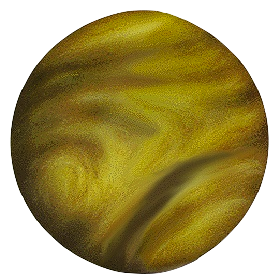
\includegraphics[width=1.2in]{images/venus.png}}

Like Planet Sample, Planet Null is a place that you construct.  You
construct it in a way that makes the Null Hypothesis true, destroying
relationships between variables.  
\authNote{R': The logical connection of the clauses in this sentence is 
unclear to me.}%
You've already seen the process in 
Section \ref{sec:comparing-two-means}: randomization with \texttt{shuffle}.
The basic idea is to treat relationships as a mapping from the values
of explanatory variables in each case to a response variable.  By
randomizing the explanatory variables relative to the response, you
generate the world in which the Null Hypothesis holds true: Planet Null. 

\subsubsection{Examples}
Let's look as some examples.

\begin{example}
The \dfn{Whickham} data set contains data from a 1970's sample of 1314
residents of Whickham,  a mixed urban and rural district near Newcastle upon Tyne, in the UK.
Did more than half of the adult residents of Whickham smoke at that time?

We could use the same approach that worked for the Lady Tasting Tea, but we'll do things 
a little differently this time.  First, let's take a quick look at some of the data.
\begin{knitrout}
\definecolor{shadecolor}{rgb}{.97, .97, .97}{\color{fgcolor}\begin{kframe}
\begin{flushleft}
\ttfamily\noindent
\hlsymbol{n}{\ }\hlassignement{\usebox{\hlnormalsizeboxlessthan}-}{\ }\hlfunctioncall{nrow}\hlkeyword{(}\hlsymbol{Whickham}\hlkeyword{)}\hspace*{\fill}\\
\hlstd{}\hlsymbol{n}\mbox{}
\normalfont
\end{flushleft}
\begin{verbatim}
[1] 1314
\end{verbatim}
\begin{flushleft}
\ttfamily\noindent
\hlfunctioncall{head}\hlkeyword{(}\hlsymbol{Whickham}\hlkeyword{,}{\ }\hlnumber{3}\hlkeyword{)}\mbox{}
\normalfont
\end{flushleft}
\begin{verbatim}
  outcome smoker age
1   Alive    Yes  23
2   Alive    Yes  18
3    Dead    Yes  71
\end{verbatim}
\end{kframe}}
\end{knitrout}

We'll answer our question by comparing the smoking rate on Planet Sample 
\begin{knitrout}
\definecolor{shadecolor}{rgb}{.97, .97, .97}{\color{fgcolor}\begin{kframe}
\begin{flushleft}
\ttfamily\noindent
\hlfunctioncall{with}\hlkeyword{(}\hlsymbol{Whickham}\hlkeyword{,}{\ }\hlfunctioncall{proptable}\hlkeyword{(}\hlsymbol{smoker}\hlkeyword{)}\hlkeyword{)}{\ }{\ }\hlcomment{\usebox{\hlnormalsizeboxhash}{\ }less{\ }than{\ }50\usebox{\hlnormalsizeboxpercent}{\ }of{\ }sample{\ }smoke}\mbox{}
\normalfont
\end{flushleft}
\begin{verbatim}
smoker
    No    Yes 
0.5571 0.4429 
\end{verbatim}
\end{kframe}}
\end{knitrout}

to the sampling distribution on Planet Null.
\begin{knitrout}
\definecolor{shadecolor}{rgb}{.97, .97, .97}{\color{fgcolor}\begin{kframe}
\begin{flushleft}
\ttfamily\noindent
\hlsymbol{planet.null}{\ }\hlassignement{\usebox{\hlnormalsizeboxlessthan}-}{\ }\hlfunctioncall{data.frame}\hlkeyword{(}\hlargument{smoker}{\ }\hlargument{=}{\ }\hlfunctioncall{c}\hlkeyword{(}\hlstring{"{}Yes"{}}\hlkeyword{,}{\ }\hlstring{"{}No"{}}\hlkeyword{)}\hlkeyword{)}{\ }{\ }\hlcomment{\usebox{\hlnormalsizeboxhash}{\ }equal{\ }mix{\ }of{\ }Yes{\ }and{\ }No{\ }on{\ }Planet{\ }Null}\hspace*{\fill}\\
\hlstd{}\hlsymbol{null.dist}{\ }\hlassignement{\usebox{\hlnormalsizeboxlessthan}-}{\ }\hlfunctioncall{do}\hlkeyword{(}\hlnumber{2000}\hlkeyword{)}{\ }\hlkeyword{*}{\ }\hlfunctioncall{with}\hlkeyword{(}\hlfunctioncall{resample}\hlkeyword{(}\hlsymbol{planet.null}\hlkeyword{,}{\ }\hlsymbol{n}\hlkeyword{)}\hlkeyword{,}{\ }\hlfunctioncall{proptable}\hlkeyword{(}\hlsymbol{smoker}\hlkeyword{)}\hlkeyword{)}\hspace*{\fill}\\
\hlstd{}\hlfunctioncall{head}\hlkeyword{(}\hlsymbol{null.dist}\hlkeyword{,}{\ }\hlnumber{3}\hlkeyword{)}\mbox{}
\normalfont
\end{flushleft}
\begin{verbatim}
      No    Yes
1 0.4848 0.5152
2 0.4878 0.5122
3 0.5084 0.4916
\end{verbatim}
\begin{flushleft}
\ttfamily\noindent
\hlfunctioncall{table}\hlkeyword{(}\hlfunctioncall{with}\hlkeyword{(}\hlsymbol{null.dist}\hlkeyword{,}{\ }\hlsymbol{Yes}{\ }\hlkeyword{\usebox{\hlnormalsizeboxlessthan}}{\ }\hlnumber{0.4429}\hlkeyword{)}\hlkeyword{)}\mbox{}
\normalfont
\end{flushleft}
\begin{verbatim}

FALSE 
 2000 
\end{verbatim}
\end{kframe}}
\end{knitrout}

2000 of our 2000 samples from Planet Null had a proportion 
of smokers smaller than the proportion on Planet Sample.  It does not appear that our 
sample came from Planet Null.
\begin{center}
\begin{knitrout}
\definecolor{shadecolor}{rgb}{.97, .97, .97}{\color{fgcolor}\begin{kframe}
\begin{flushleft}
\ttfamily\noindent
\hlfunctioncall{histogram}\hlkeyword{(}\hlkeyword{\urltilda{}}\hlsymbol{Yes}\hlkeyword{,}{\ }\hlsymbol{null.dist}\hlkeyword{,}{\ }\hlargument{main}{\ }\hlargument{=}{\ }\hlstring{"{}Sampling{\ }distribution{\ }of{\ }smoking{\ }proportion"{}}\hlkeyword{)}\mbox{}
\normalfont
\end{flushleft}


\centering{}\includegraphics{figures/fig-Whickham-smokers} 

\end{kframe}}
\end{knitrout}

\end{center}
\end{example}

\begin{example}
Do the foot widths differ between boys and girls, judging from
the \texttt{KidsFeet} data?
\begin{knitrout}
\definecolor{shadecolor}{rgb}{.97, .97, .97}{\color{fgcolor}\begin{kframe}
\begin{flushleft}
\ttfamily\noindent
\hlfunctioncall{data}\hlkeyword{(}\hlsymbol{KidsFeet}\hlkeyword{)}\hspace*{\fill}\\
\hlstd{}\hlfunctioncall{lm}\hlkeyword{(}\hlsymbol{width}{\ }\hlkeyword{\urltilda{}}{\ }\hlsymbol{sex}\hlkeyword{,}{\ }\hlargument{data}{\ }\hlargument{=}{\ }\hlsymbol{KidsFeet}\hlkeyword{)}{\ }{\ }\hlcomment{\usebox{\hlnormalsizeboxhash}{\ }our{\ }sample}\mbox{}
\normalfont
\end{flushleft}
\begin{verbatim}

Call:
lm(formula = width ~ sex, data = KidsFeet)

Coefficients:
(Intercept)         sexG  
      9.190       -0.406  

\end{verbatim}
\end{kframe}}
\end{knitrout}

\FoodForThought{Conceptually, this example can be done without the use of \function{lm()},
but the syntax is trickier.  \function{lm()} takes care of computing the means of the two
groups and the difference in those means.  See Section~\ref{sec:comparing-two-means}.}%
\authNote{rjp: I installed local copies of \function{print.lm()} and \function{print.summary.lm()}
in \texttt{setup.R}, so at least in this document, the extra clutter is gone.}%
\authNoted{DTK: What do you say we re-define display.lm in the mosaic
  package to get rid of the report about the Call.  It just takes up
  useless space.}
Looks like girls' feet are a little bit narrower.  But is this the
sort of thing we might equally well see on Planet Null, where there is
no systematic difference between boys' and girls' feet?


\begin{knitrout}
\definecolor{shadecolor}{rgb}{.97, .97, .97}{\color{fgcolor}\begin{kframe}
\begin{flushleft}
\ttfamily\noindent
\hlfunctioncall{do}\hlkeyword{(}\hlnumber{1}\hlkeyword{)}{\ }\hlkeyword{*}{\ }\hlfunctioncall{lm}\hlkeyword{(}\hlsymbol{width}{\ }\hlkeyword{\urltilda{}}{\ }\hlfunctioncall{shuffle}\hlkeyword{(}\hlsymbol{sex}\hlkeyword{)}\hlkeyword{,}{\ }\hlargument{data}{\ }\hlargument{=}{\ }\hlsymbol{KidsFeet}\hlkeyword{)}{\ }{\ }\hlcomment{\usebox{\hlnormalsizeboxhash}{\ }planet{\ }null}\mbox{}
\normalfont
\end{flushleft}
\begin{verbatim}
  Intercept   sexG  sigma r-squared
1      8.92 0.1484 0.5108   0.02175
\end{verbatim}
\end{kframe}}
\end{knitrout}

For this particular sample from Planet Null, the girls' feet are a
little wider than the boys'.  By generating a sampling distribution on
Planet Null, we can see the size of the relationship to be expected
just due to sampling fluctuations in a world where there is no relationship.
\begin{knitrout}
\definecolor{shadecolor}{rgb}{.97, .97, .97}{\color{fgcolor}\begin{kframe}
\begin{flushleft}
\ttfamily\noindent
\hlcomment{\usebox{\hlnormalsizeboxhash}{\ }(approximate){\ }distribution{\ }on{\ }planet{\ }null}\hspace*{\fill}\\
\hlstd{}\hlsymbol{planet.null}{\ }\hlassignement{\usebox{\hlnormalsizeboxlessthan}-}{\ }\hlfunctioncall{do}\hlkeyword{(}\hlnumber{500}\hlkeyword{)}{\ }\hlkeyword{*}{\ }\hlfunctioncall{lm}\hlkeyword{(}\hlsymbol{width}{\ }\hlkeyword{\urltilda{}}{\ }\hlfunctioncall{shuffle}\hlkeyword{(}\hlsymbol{sex}\hlkeyword{)}\hlkeyword{,}{\ }\hlargument{data}{\ }\hlargument{=}{\ }\hlsymbol{KidsFeet}\hlkeyword{)}\hspace*{\fill}\\
\hlstd{}\hlfunctioncall{head}\hlkeyword{(}\hlsymbol{planet.null}\hlkeyword{,}{\ }\hlnumber{2}\hlkeyword{)}\mbox{}
\normalfont
\end{flushleft}
\begin{verbatim}
  Intercept   sexG  sigma r-squared
1     8.815 0.3639 0.4815   0.13079
2     8.940 0.1074 0.5135   0.01138
\end{verbatim}
\end{kframe}}
\end{knitrout}

\begin{knitrout}
\definecolor{shadecolor}{rgb}{.97, .97, .97}{\color{fgcolor}\begin{kframe}
\begin{flushleft}
\ttfamily\noindent
\hlfunctioncall{with}\hlkeyword{(}\hlsymbol{planet.null}\hlkeyword{,}{\ }\hlfunctioncall{mean}\hlkeyword{(}\hlfunctioncall{abs}\hlkeyword{(}\hlsymbol{sexG}\hlkeyword{)}{\ }\hlkeyword{\usebox{\hlnormalsizeboxgreaterthan}}{\ }\hlfunctioncall{abs}\hlkeyword{(}\hlkeyword{-}\hlnumber{0.4058}\hlkeyword{)}\hlkeyword{)}\hlkeyword{)}{\ }{\ }\hlcomment{\usebox{\hlnormalsizeboxhash}{\ }a{\ }p-value}\mbox{}
\normalfont
\end{flushleft}
\begin{verbatim}
 mean 
0.012 
\end{verbatim}
\end{kframe}}
\end{knitrout}

The value of $-0.4058$ observed in our sample is not very likely on
Planet Null.  This suggests that our sample was not collected from
Planet Null: we can reject the Null Hypothesis.

%\InstructorNote{The \texttt{[,2]} means to take the 2nd column of \texttt{sn1}. }
%\authNote{If we can suppress the shuffle in the output of do(), then
%  we can just use the \$ notation for pulling out a column.}

\end{example}

\begin{example}
Is the survival rate for smokers different from that for non-smokers?
\begin{knitrout}
\definecolor{shadecolor}{rgb}{.97, .97, .97}{\color{fgcolor}\begin{kframe}
\begin{flushleft}
\ttfamily\noindent
\hlfunctioncall{do}\hlkeyword{(}\hlnumber{1}\hlkeyword{)}{\ }\hlkeyword{*}{\ }\hlfunctioncall{lm}\hlkeyword{(}\hlsymbol{outcome}{\ }=={\ }\hlstring{"{}Alive"{}}{\ }\hlkeyword{\urltilda{}}{\ }\hlsymbol{smoker}\hlkeyword{,}{\ }\hlargument{data}{\ }\hlargument{=}{\ }\hlsymbol{Whickham}\hlkeyword{)}{\ }{\ }\hlcomment{\usebox{\hlnormalsizeboxhash}{\ }from{\ }our{\ }sample}\mbox{}
\normalfont
\end{flushleft}
\begin{verbatim}
  Intercept smokerYes  sigma r-squared
1    0.6858   0.07538 0.4482  0.006941
\end{verbatim}
\begin{flushleft}
\ttfamily\noindent
\hlfunctioncall{do}\hlkeyword{(}\hlnumber{1}\hlkeyword{)}{\ }\hlkeyword{*}{\ }\hlfunctioncall{lm}\hlkeyword{(}\hlsymbol{outcome}{\ }=={\ }\hlstring{"{}Alive"{}}{\ }\hlkeyword{\urltilda{}}{\ }\hlfunctioncall{shuffle}\hlkeyword{(}\hlsymbol{smoker}\hlkeyword{)}\hlkeyword{,}{\ }\hlargument{data}{\ }\hlargument{=}{\ }\hlsymbol{Whickham}\hlkeyword{)}{\ }{\ }\hlcomment{\usebox{\hlnormalsizeboxhash}{\ }planet{\ }null}\mbox{}
\normalfont
\end{flushleft}
\begin{verbatim}
  Intercept smokerYes  sigma r-squared
1    0.7145   0.01061 0.4497 0.0001374
\end{verbatim}
\begin{flushleft}
\ttfamily\noindent
\hlcomment{\usebox{\hlnormalsizeboxhash}{\ }distribution{\ }on{\ }planet{\ }null}\hspace*{\fill}\\
\hlstd{}\hlsymbol{null.distribution}{\ }\hlassignement{=}{\ }\hlfunctioncall{do}\hlkeyword{(}\hlnumber{500}\hlkeyword{)}{\ }\hlkeyword{*}{\ }\hlfunctioncall{lm}\hlkeyword{(}\hlsymbol{outcome}{\ }=={\ }\hlstring{"{}Alive"{}}{\ }\hlkeyword{\urltilda{}}{\ }\hlfunctioncall{shuffle}\hlkeyword{(}\hlsymbol{smoker}\hlkeyword{)}\hlkeyword{,}\hspace*{\fill}\\
\hlstd{}{\ }{\ }{\ }{\ }\hlargument{data}{\ }\hlargument{=}{\ }\hlsymbol{Whickham}\hlkeyword{)}\hspace*{\fill}\\
\hlstd{}\hlfunctioncall{with}\hlkeyword{(}\hlsymbol{null.distribution}\hlkeyword{,}{\ }\hlfunctioncall{mean}\hlkeyword{(}\hlfunctioncall{abs}\hlkeyword{(}\hlsymbol{smokerYes}\hlkeyword{)}{\ }\hlkeyword{\usebox{\hlnormalsizeboxgreaterthan}}{\ }\hlfunctioncall{abs}\hlkeyword{(}\hlnumber{0.07538}\hlkeyword{)}\hlkeyword{)}\hlkeyword{)}{\ }{\ }\hlcomment{\usebox{\hlnormalsizeboxhash}{\ }a{\ }p-value}\mbox{}
\normalfont
\end{flushleft}
\begin{verbatim}
mean 
   0 
\end{verbatim}
\end{kframe}}
\end{knitrout}

If you're shocked to see that smoking is associated with greater
likelihood of being alive (7.5 percentage points greater!) and that
the data indicate that this is statistically significant, you should
be.  But the problem isn't with the calculation, which is the same one
you will get from the textbook formulas.  The problem is with the
failure to take into account covariates.  What's shocking is that we
teach students about p-values without teaching them about covariates
and how to adjust for them.


The big covariate here is \VN{age}.  It happens that in the Whickham
 data, younger people are more likely to smoke.  To see this you :
\begin{knitrout}
\definecolor{shadecolor}{rgb}{.97, .97, .97}{\color{fgcolor}\begin{kframe}
\begin{flushleft}
\ttfamily\noindent
\hlfunctioncall{do}\hlkeyword{(}\hlnumber{1}\hlkeyword{)}{\ }\hlkeyword{*}{\ }\hlfunctioncall{lm}\hlkeyword{(}\hlsymbol{smoker}{\ }=={\ }\hlstring{"{}Yes"{}}{\ }\hlkeyword{\urltilda{}}{\ }\hlsymbol{age}\hlkeyword{,}{\ }\hlargument{data}{\ }\hlargument{=}{\ }\hlsymbol{Whickham}\hlkeyword{)}{\ }{\ }\hlcomment{\usebox{\hlnormalsizeboxhash}{\ }our{\ }sample}\mbox{}
\normalfont
\end{flushleft}
\begin{verbatim}
  Intercept       age  sigma r-squared
1    0.5961 -0.003264 0.4938   0.01311
\end{verbatim}
\begin{flushleft}
\ttfamily\noindent
\hlfunctioncall{do}\hlkeyword{(}\hlnumber{1}\hlkeyword{)}{\ }\hlkeyword{*}{\ }\hlfunctioncall{lm}\hlkeyword{(}\hlsymbol{smoker}{\ }=={\ }\hlstring{"{}Yes"{}}{\ }\hlkeyword{\urltilda{}}{\ }\hlfunctioncall{shuffle}\hlkeyword{(}\hlsymbol{age}\hlkeyword{)}\hlkeyword{,}{\ }\hlargument{data}{\ }\hlargument{=}{\ }\hlsymbol{Whickham}\hlkeyword{)}{\ }{\ }\hlcomment{\usebox{\hlnormalsizeboxhash}{\ }under{\ }the{\ }null}\mbox{}
\normalfont
\end{flushleft}
\begin{verbatim}
  Intercept        age sigma r-squared
1    0.4694 -0.0005652 0.497 0.0003931
\end{verbatim}
\begin{flushleft}
\ttfamily\noindent
\hlcomment{\usebox{\hlnormalsizeboxhash}{\ }distribution{\ }on{\ }planet{\ }null}\hspace*{\fill}\\
\hlstd{}\hlsymbol{null.distribution}{\ }\hlassignement{\usebox{\hlnormalsizeboxlessthan}-}{\ }\hlfunctioncall{do}\hlkeyword{(}\hlnumber{500}\hlkeyword{)}{\ }\hlkeyword{*}{\ }\hlfunctioncall{lm}\hlkeyword{(}\hlsymbol{smoker}{\ }=={\ }\hlstring{"{}Yes"{}}{\ }\hlkeyword{\urltilda{}}{\ }\hlfunctioncall{shuffle}\hlkeyword{(}\hlsymbol{age}\hlkeyword{)}\hlkeyword{,}\hspace*{\fill}\\
\hlstd{}{\ }{\ }{\ }{\ }\hlargument{data}{\ }\hlargument{=}{\ }\hlsymbol{Whickham}\hlkeyword{)}\hspace*{\fill}\\
\hlstd{}\hlfunctioncall{with}\hlkeyword{(}\hlsymbol{null.distribution}\hlkeyword{,}{\ }\hlfunctioncall{mean}\hlkeyword{(}\hlfunctioncall{abs}\hlkeyword{(}\hlsymbol{age}\hlkeyword{)}{\ }\hlkeyword{\usebox{\hlnormalsizeboxgreaterthan}}{\ }\hlfunctioncall{abs}\hlkeyword{(}\hlkeyword{-}\hlnumber{0.00326}\hlkeyword{)}\hlkeyword{)}\hlkeyword{)}{\ }{\ }\hlcomment{\usebox{\hlnormalsizeboxhash}{\ }approx.{\ }p-value}\mbox{}
\normalfont
\end{flushleft}
\begin{verbatim}
mean 
   0 
\end{verbatim}
\end{kframe}}
\end{knitrout}

So, greater \VN{age} is associated with lower \VN{smoker} status.
And, of course, older people  are more likely to die.  Taking both factors
together, it turns out that smokers are less likely to die, but that's because
they are young.  
\end{example}

\begin{example}
Let's make up for the deficiency in the above smoking example.
One way to do this is to adjust for \VN{age} when considering the
effect of \VN{smoker} status.  We'll consider this more in Chapter
\ref{chap:Multivariate-early}, but for now, we'll just build the model.
  
\begin{knitrout}
\definecolor{shadecolor}{rgb}{.97, .97, .97}{\color{fgcolor}\begin{kframe}
\begin{flushleft}
\ttfamily\noindent
\hlcomment{\usebox{\hlnormalsizeboxhash}{\ }our{\ }sample{\ }on{\ }planet{\ }Earth}\hspace*{\fill}\\
\hlstd{}\hlfunctioncall{do}\hlkeyword{(}\hlnumber{1}\hlkeyword{)}{\ }\hlkeyword{*}{\ }\hlfunctioncall{glm}\hlkeyword{(}\hlsymbol{outcome}{\ }=={\ }\hlstring{"{}Alive"{}}{\ }\hlkeyword{\urltilda{}}{\ }\hlsymbol{smoker}{\ }\hlkeyword{+}{\ }\hlsymbol{age}\hlkeyword{,}{\ }\hlargument{data}{\ }\hlargument{=}{\ }\hlsymbol{Whickham}\hlkeyword{,}{\ }\hlargument{family}{\ }\hlargument{=}{\ }\hlstring{"{}binomial"{}}\hlkeyword{)}\mbox{}
\normalfont
\end{flushleft}
\begin{verbatim}
  Intercept smokerYes     age
1     7.599   -0.2047 -0.1237
\end{verbatim}
\begin{flushleft}
\ttfamily\noindent
\hlcomment{\usebox{\hlnormalsizeboxhash}{\ }o{\ }sample{\ }on{\ }planet{\ }null}\hspace*{\fill}\\
\hlstd{}\hlfunctioncall{do}\hlkeyword{(}\hlnumber{1}\hlkeyword{)}{\ }\hlkeyword{*}{\ }\hlfunctioncall{glm}\hlkeyword{(}\hlsymbol{outcome}{\ }=={\ }\hlstring{"{}Alive"{}}{\ }\hlkeyword{\urltilda{}}{\ }\hlfunctioncall{shuffle}\hlkeyword{(}\hlsymbol{smoker}\hlkeyword{)}{\ }\hlkeyword{+}{\ }\hlsymbol{age}\hlkeyword{,}{\ }\hlargument{data}{\ }\hlargument{=}{\ }\hlsymbol{Whickham}\hlkeyword{,}\hspace*{\fill}\\
\hlstd{}{\ }{\ }{\ }{\ }\hlargument{family}{\ }\hlargument{=}{\ }\hlstring{"{}binomial"{}}\hlkeyword{)}\mbox{}
\normalfont
\end{flushleft}
\begin{verbatim}
  Intercept smokerYes     age
1     7.393   0.02131 -0.1219
\end{verbatim}
\begin{flushleft}
\ttfamily\noindent
\hlcomment{\usebox{\hlnormalsizeboxhash}{\ }distribution{\ }on{\ }planet{\ }null}\hspace*{\fill}\\
\hlstd{}\hlsymbol{null.distribution}{\ }\hlassignement{\usebox{\hlnormalsizeboxlessthan}-}{\ }\hlfunctioncall{do}\hlkeyword{(}\hlnumber{500}\hlkeyword{)}{\ }\hlkeyword{*}{\ }\hlfunctioncall{glm}\hlkeyword{(}\hlsymbol{outcome}{\ }=={\ }\hlstring{"{}Alive"{}}{\ }\hlkeyword{\urltilda{}}{\ }\hlfunctioncall{shuffle}\hlkeyword{(}\hlsymbol{smoker}\hlkeyword{)}{\ }\hlkeyword{+}\hspace*{\fill}\\
\hlstd{}{\ }{\ }{\ }{\ }\hlsymbol{age}\hlkeyword{,}{\ }\hlargument{data}{\ }\hlargument{=}{\ }\hlsymbol{Whickham}\hlkeyword{,}{\ }\hlargument{family}{\ }\hlargument{=}{\ }\hlstring{"{}binomial"{}}\hlkeyword{)}\hspace*{\fill}\\
\hlstd{}\hlfunctioncall{with}\hlkeyword{(}\hlsymbol{null.distribution}\hlkeyword{,}{\ }\hlfunctioncall{mean}\hlkeyword{(}\hlfunctioncall{abs}\hlkeyword{(}\hlsymbol{smokerYes}\hlkeyword{)}{\ }\hlkeyword{\usebox{\hlnormalsizeboxgreaterthan}}{\ }\hlfunctioncall{abs}\hlkeyword{(}\hlkeyword{-}\hlnumber{0.205}\hlkeyword{)}\hlkeyword{)}\hlkeyword{)}{\ }{\ }\hlcomment{\usebox{\hlnormalsizeboxhash}{\ }approx.{\ }p-value}\mbox{}
\normalfont
\end{flushleft}
\begin{verbatim}
 mean 
0.222 
\end{verbatim}
\end{kframe}}
\end{knitrout}

You can see that the coefficient on \texttt{smokerYes} is negative,
and that the p-value indicates significance.  So, smoking in these
data are associated with a lower probability of survival, but only
when adjusting for \VN{age}.

You might have noticed that the model built here was a logistic
model.  There's good reason to do that, since we are modeling
probabilities the value of which must always be between 0 and 1.  But
notice also that the logic of hypothesis testing remains the same:
construct a Planet Null by randomizing an explanatory variable with
respect to a response variable.
\end{example}

As this is being written, the US Space Shuttle is carrying out it's
last couple of missions before being retired.  For a few years, at
least, your students will know what you mean by ``Space Shuttle.''
You can help them remember the way to create Planet Null if, at the
cost of some self-dignity, you tell them, ``Take the Space Shuffle to
Planet Null.''


\subsection{The Sampling Distribution Under the Alternative Hypothesis}

Planet Alt is the place where we implement our theories of how the
world works.  This will seem like an odd statement to those who are
familiar with the standard introductory textbook formulation of the
alternative hypothesis in its ``anything  but the Null'' form, e.g.,
$H_a : \mu_1 \neq \mu_2$.  Move away from that formulation, whose only
point seems to be to inform whether to do a one-tailed or a two-tailed test.

Instead head off to Planet Alt.

\centerline{
\includegraphics[width=1.2in]{images/planet-alt.png}}

How do you get there?  You build a simulation of the world as you
think it might be.  

\begin{example}
To illustrate, imagine that you are interested in
researching the potential relationship between vitamin D deficiency
and high blood pressure.  Your eventual plan is to do a study, perhaps
one where you draw blood samples to measure vitamin D levels, and
correlate this with high blood pressure.  From your previous
experience, you know that high blood pressure is particularly a problem in men aged
50 and older, and that black men seem to be more susceptible than
whites.

You scour the literature, looking for data on vitaminD and blood
pressure.  What you find are some papers describing vitamin D levels
in blacks and whites, and that, on average, blacks seem to have substantially lower
vitamin D levels than whites.  There's also data on high blood
pressure, but no good study relating vitamin D to blood pressure.
That's a problem, but it's also the source of your research opportunity.

You form your alternative hypothesis based on your idea of a world in
which the relationship between vitamin D and blood pressure is large
enough to be interesting at a clinical level, but small enough to have
been missed by past research.  You decide a substantial but typical
deficiency in vitamin D will, on average lead to a 5mmHg increase in
systolic blood pressure.

\InstructorNote{The instructor would
  provide this function to the students.}

Now, to construct Planet Alt: 
\begin{knitrout}
\definecolor{shadecolor}{rgb}{.97, .97, .97}{\color{fgcolor}\begin{kframe}
\begin{flushleft}
\ttfamily\noindent
\hlsymbol{planet.alt}{\ }\hlassignement{=}{\ }\hlkeyword{function}\hlkeyword{(}\hlformalargs{n}{\ }\hleqformalargs{=}{\ }\hlnumber{10}\hlkeyword{,}{\ }\hlformalargs{effect.size}{\ }\hleqformalargs{=}{\ }\hlnumber{1}\hlkeyword{)}{\ }\hlkeyword{\usebox{\hlnormalsizeboxopenbrace}}\hspace*{\fill}\\
\hlstd{}{\ }{\ }{\ }{\ }\hlsymbol{race}{\ }\hlassignement{=}{\ }\hlfunctioncall{resample}\hlkeyword{(}\hlfunctioncall{c}\hlkeyword{(}\hlstring{"{}B"{}}\hlkeyword{,}{\ }\hlstring{"{}B"{}}\hlkeyword{,}{\ }\hlstring{"{}W"{}}\hlkeyword{,}{\ }\hlstring{"{}W"{}}\hlkeyword{,}{\ }\hlstring{"{}W"{}}\hlkeyword{)}\hlkeyword{,}{\ }\hlsymbol{n}\hlkeyword{)}\hspace*{\fill}\\
\hlstd{}{\ }{\ }{\ }{\ }\hlsymbol{D}{\ }\hlassignement{=}{\ }\hlfunctioncall{pmax}\hlkeyword{(}\hlnumber{0}\hlkeyword{,}{\ }\hlfunctioncall{rnorm}\hlkeyword{(}\hlsymbol{n}\hlkeyword{,}{\ }\hlargument{mean}{\ }\hlargument{=}{\ }\hlkeyword{(}\hlnumber{37.7}{\ }\hlkeyword{+}{\ }\hlkeyword{(}\hlnumber{71.8}{\ }\hlkeyword{-}{\ }\hlnumber{37.7}\hlkeyword{)}{\ }\hlkeyword{*}{\ }\hlkeyword{(}\hlsymbol{race}{\ }=={\ }\hlstring{"{}W"{}}\hlkeyword{)}\hlkeyword{)}\hlkeyword{,}{\ }\hlargument{sd}{\ }\hlargument{=}{\ }\hlkeyword{(}\hlnumber{10}{\ }\hlkeyword{+}\hspace*{\fill}\\
\hlstd{}{\ }{\ }{\ }{\ }{\ }{\ }{\ }{\ }\hlkeyword{(}\hlnumber{20}{\ }\hlkeyword{-}{\ }\hlnumber{10}\hlkeyword{)}{\ }\hlkeyword{*}{\ }\hlkeyword{(}\hlsymbol{race}{\ }=={\ }\hlstring{"{}W"{}}\hlkeyword{)}\hlkeyword{)}\hlkeyword{)}\hlkeyword{)}\hspace*{\fill}\\
\hlstd{}{\ }{\ }{\ }{\ }\hlsymbol{systolic}{\ }\hlassignement{=}{\ }\hlfunctioncall{pmax}\hlkeyword{(}\hlnumber{80}\hlkeyword{,}{\ }\hlfunctioncall{rnorm}\hlkeyword{(}\hlsymbol{n}\hlkeyword{,}{\ }\hlargument{mean}{\ }\hlargument{=}{\ }\hlnumber{130}\hlkeyword{,}{\ }\hlargument{sd}{\ }\hlargument{=}{\ }\hlnumber{8}\hlkeyword{)}{\ }\hlkeyword{+}{\ }\hlfunctioncall{rexp}\hlkeyword{(}\hlsymbol{n}\hlkeyword{,}{\ }\hlargument{rate}{\ }\hlargument{=}{\ }\hlnumber{0.15}\hlkeyword{)}{\ }\hlkeyword{+}\hspace*{\fill}\\
\hlstd{}{\ }{\ }{\ }{\ }{\ }{\ }{\ }{\ }\hlsymbol{effect.size}{\ }\hlkeyword{*}{\ }\hlkeyword{(}\hlnumber{30}{\ }\hlkeyword{-}{\ }\hlsymbol{D}\hlkeyword{)}\hlkeyword{/}\hlnumber{2}\hlkeyword{)}\hspace*{\fill}\\
\hlstd{}{\ }{\ }{\ }{\ }\hlfunctioncall{return}\hlkeyword{(}\hlfunctioncall{data.frame}\hlkeyword{(}\hlargument{race}{\ }\hlargument{=}{\ }\hlsymbol{race}\hlkeyword{,}{\ }\hlargument{D}{\ }\hlargument{=}{\ }\hlsymbol{D}\hlkeyword{,}{\ }\hlargument{systolic}{\ }\hlargument{=}{\ }\hlfunctioncall{round}\hlkeyword{(}\hlsymbol{systolic}\hlkeyword{)}\hlkeyword{)}\hlkeyword{)}\hspace*{\fill}\\
\hlstd{}\hlkeyword{\usebox{\hlnormalsizeboxclosebrace}}\mbox{}
\normalfont
\end{flushleft}
\end{kframe}}
\end{knitrout}

The internals of such a function is not for the faint of heart.  You'll see that it
creates people that are randomly of race B or W, and in a proportion
that you might choose if you were sampling with the intent of
examining seriously the role that race plays.  The vitamin D level is
set, according to your findings in the literature, to have a mean of
37.7 for blacks and 71.8 for whites.  The standard deviations also
differ between blacks and whites.  Finally, the systolic blood is set
to produce a population that is a mixture of a normal distribution
around 130 mmHg with an exponential tail toward high blood pressure. 
A drop of vitaminD levels of 10 units leads to an increase in blood
pressure of 5 mmHg.  There's a parameter, \texttt{effect.size} that
will allow you to change this without re-programming.

You might not agree with this specific alternative hypothesis.  That's
fine.  You can make your own Planet Alt.  There are plenty to go around!

In contrast to the complexity of writing the simulation, using it is
simple.  Here's a quick study of size $n=5$:
\begin{knitrout}
\definecolor{shadecolor}{rgb}{.97, .97, .97}{\color{fgcolor}\begin{kframe}
\begin{flushleft}
\ttfamily\noindent
\hlfunctioncall{planet.alt}\hlkeyword{(}\hlnumber{5}\hlkeyword{)}\mbox{}
\normalfont
\end{flushleft}
\begin{verbatim}
  race     D systolic
1    W 54.28      118
2    B 45.09      126
3    B 23.74      136
4    B 48.27      139
5    B 34.91      137
\end{verbatim}
\end{kframe}}
\end{knitrout}

\end{example}

\begin{example}
In this example we construct Planet Alt for a comparison of two means.
\begin{knitrout}
\definecolor{shadecolor}{rgb}{.97, .97, .97}{\color{fgcolor}\begin{kframe}
\begin{flushleft}
\ttfamily\noindent
\hlsymbol{alt.2.groups}{\ }\hlassignement{\usebox{\hlnormalsizeboxlessthan}-}{\ }\hlkeyword{function}\hlkeyword{(}\hlformalargs{n}{\ }\hleqformalargs{=}{\ }\hlnumber{10}\hlkeyword{,}{\ }\hlformalargs{effect.size}{\ }\hleqformalargs{=}{\ }\hlnumber{1}\hlkeyword{,}{\ }\hlformalargs{sd}{\ }\hleqformalargs{=}{\ }\hlnumber{1}\hlkeyword{,}{\ }\hlformalargs{baseline}{\ }\hleqformalargs{=}{\ }\hlnumber{0}\hlkeyword{)}{\ }\hlkeyword{\usebox{\hlnormalsizeboxopenbrace}}\hspace*{\fill}\\
\hlstd{}{\ }{\ }{\ }{\ }\hlsymbol{n}{\ }\hlassignement{\usebox{\hlnormalsizeboxlessthan}-}{\ }\hlfunctioncall{rep}\hlkeyword{(}\hlsymbol{n}\hlkeyword{,}{\ }\hlargument{length.out}{\ }\hlargument{=}{\ }\hlnumber{2}\hlkeyword{)}\hspace*{\fill}\\
\hlstd{}{\ }{\ }{\ }{\ }\hlsymbol{sd}{\ }\hlassignement{\usebox{\hlnormalsizeboxlessthan}-}{\ }\hlfunctioncall{rep}\hlkeyword{(}\hlsymbol{sd}\hlkeyword{,}{\ }\hlargument{length.out}{\ }\hlargument{=}{\ }\hlnumber{2}\hlkeyword{)}\hspace*{\fill}\\
\hlstd{}{\ }{\ }{\ }{\ }\hlfunctioncall{data.frame}\hlkeyword{(}\hlargument{y}{\ }\hlargument{=}{\ }\hlfunctioncall{c}\hlkeyword{(}\hlfunctioncall{rnorm}\hlkeyword{(}\hlsymbol{n}\hlkeyword{[}\hlnumber{1}\hlkeyword{]}\hlkeyword{,}{\ }\hlsymbol{baseline}\hlkeyword{,}{\ }\hlsymbol{sd}\hlkeyword{[}\hlnumber{1}\hlkeyword{]}\hlkeyword{)}\hlkeyword{,}{\ }\hlfunctioncall{rnorm}\hlkeyword{(}\hlsymbol{n}\hlkeyword{[}\hlnumber{2}\hlkeyword{]}\hlkeyword{,}{\ }\hlsymbol{baseline}{\ }\hlkeyword{+}{\ }\hlsymbol{effect.size}\hlkeyword{,}\hspace*{\fill}\\
\hlstd{}{\ }{\ }{\ }{\ }{\ }{\ }{\ }{\ }\hlsymbol{sd}\hlkeyword{[}\hlnumber{2}\hlkeyword{]}\hlkeyword{)}\hlkeyword{)}\hlkeyword{,}{\ }\hlargument{group}{\ }\hlargument{=}{\ }\hlfunctioncall{rep}\hlkeyword{(}\hlfunctioncall{c}\hlkeyword{(}\hlstring{"{}A"{}}\hlkeyword{,}{\ }\hlstring{"{}B"{}}\hlkeyword{)}\hlkeyword{,}{\ }\hlsymbol{n}\hlkeyword{)}\hlkeyword{)}\hspace*{\fill}\\
\hlstd{}\hlkeyword{\usebox{\hlnormalsizeboxclosebrace}}\mbox{}
\normalfont
\end{flushleft}
\end{kframe}}
\end{knitrout}

\begin{knitrout}
\definecolor{shadecolor}{rgb}{.97, .97, .97}{\color{fgcolor}\begin{kframe}
\begin{flushleft}
\ttfamily\noindent
\hlfunctioncall{alt.2.groups}\hlkeyword{(}\hlnumber{3}\hlkeyword{)}\mbox{}
\normalfont
\end{flushleft}
\begin{verbatim}
        y group
1 -0.5794     A
2 -0.5298     A
3  0.6280     A
4 -0.3159     B
5 -0.5045     B
6  0.1617     B
\end{verbatim}
\end{kframe}}
\end{knitrout}

\end{example}

We'll discuss how to use such simulations to compute power in Section \ref{sec:power}.

\begin{problem}
\begin{enumerate}
\item   Write an alternative-hypothesis simulation where there are two groups: A and B.  In your
  alternative hypothesis, the population mean of A is 90 and the
  population mean of B is 110.  Let the standard deviation be 30 for
  group A and 35 for group B.  
 
\item You've got two different suppliers of electronic components, C
  and D.
  You hypothesize that one of them, D, is somewhat defective. Their
  components have a lifetime that's distributed exponentially with a
  mean lifetime of 1000.  Supplier C is better, you think, and meets
  the specified mean lifetime of 2000.  
  
  Write an alternative hypothesis simulation of the two suppliers.
\end{enumerate}  
\end{problem}

\section{More Examples}

\subsection{Comparing Two Means}

\label{sec:comparing-two-means}

In this section we show several ways to see if the mean ages of men and women in the HELP study 
are significantly different.



\subsubsection{Using \texttt{lm()}}
\label{sec:lm}
We begin with a simple method that uses a big tool -- linear models.  If you do 
linear models early, this is the way to go.


In this example, \R\ will automatically convert the \variable{sex} factor into
0's and 1's, so the slope parameter in the model is the difference in the means.  
\begin{knitrout}
\definecolor{shadecolor}{rgb}{.97, .97, .97}{\color{fgcolor}\begin{kframe}
\begin{flushleft}
\ttfamily\noindent
\hlfunctioncall{mean}\hlkeyword{(}\hlsymbol{age}{\ }\hlkeyword{\urltilda{}}{\ }\hlsymbol{sex}\hlkeyword{,}{\ }\hlargument{data}{\ }\hlargument{=}{\ }\hlsymbol{HELP}\hlkeyword{)}\mbox{}
\normalfont
\end{flushleft}
\begin{verbatim}
     sex     S   N Missing
1 female 36.25 107       0
2   male 35.47 346       0
\end{verbatim}
\begin{flushleft}
\ttfamily\noindent
\hlfunctioncall{lm}\hlkeyword{(}\hlsymbol{age}{\ }\hlkeyword{\urltilda{}}{\ }\hlsymbol{sex}\hlkeyword{,}{\ }\hlargument{data}{\ }\hlargument{=}{\ }\hlsymbol{HELP}\hlkeyword{)}{\ }{\ }\hlcomment{\usebox{\hlnormalsizeboxhash}{\ }actual{\ }data}\mbox{}
\normalfont
\end{flushleft}
\begin{verbatim}

Call:
lm(formula = age ~ sex, data = HELP)

Coefficients:
(Intercept)      sexmale  
     36.252       -0.784  

\end{verbatim}
\end{kframe}}
\end{knitrout}

The \function{do()} function conveniently stores the values of the 
estimated parameters that result from fitting with \function{lm()}, 
so it is relatively easy to obtain
the sampling distribution for any of these estimated parameters.
\begin{knitrout}
\definecolor{shadecolor}{rgb}{.97, .97, .97}{\color{fgcolor}\begin{kframe}
\begin{flushleft}
\ttfamily\noindent
\hlfunctioncall{do}\hlkeyword{(}\hlnumber{1}\hlkeyword{)}{\ }\hlkeyword{*}{\ }\hlfunctioncall{lm}\hlkeyword{(}\hlsymbol{age}{\ }\hlkeyword{\urltilda{}}{\ }\hlsymbol{sex}\hlkeyword{,}{\ }\hlargument{data}{\ }\hlargument{=}{\ }\hlsymbol{HELP}\hlkeyword{)}{\ }{\ }\hlcomment{\usebox{\hlnormalsizeboxhash}{\ }actual{\ }data}\mbox{}
\normalfont
\end{flushleft}
\begin{verbatim}
  Intercept sexmale sigma r-squared
1     36.25 -0.7841 7.712   0.00187
\end{verbatim}
\begin{flushleft}
\ttfamily\noindent
\hlfunctioncall{do}\hlkeyword{(}\hlnumber{2}\hlkeyword{)}{\ }\hlkeyword{*}{\ }\hlfunctioncall{lm}\hlkeyword{(}\hlsymbol{age}{\ }\hlkeyword{\urltilda{}}{\ }\hlfunctioncall{shuffle}\hlkeyword{(}\hlsymbol{sex}\hlkeyword{)}\hlkeyword{,}{\ }\hlargument{data}{\ }\hlargument{=}{\ }\hlsymbol{HELP}\hlkeyword{)}{\ }{\ }\hlcomment{\usebox{\hlnormalsizeboxhash}{\ }shuffled{\ }data}\mbox{}
\normalfont
\end{flushleft}
\begin{verbatim}
  Intercept sexmale sigma r-squared
1     34.54   1.455 7.694  0.006439
2     34.69   1.259 7.700  0.004823
\end{verbatim}
\end{kframe}}
\end{knitrout}


%Since this is just another way of computing the difference in the sample means, the two approaches
%are equivalent.  If we reset the random seed, we get exactly the same simulation results.
\begin{knitrout}
\definecolor{shadecolor}{rgb}{.97, .97, .97}{\color{fgcolor}\begin{kframe}
\begin{flushleft}
\ttfamily\noindent
\hlfunctioncall{set.seed}\hlkeyword{(}\hlnumber{123}\hlkeyword{)}{\ }{\ }\hlcomment{\usebox{\hlnormalsizeboxhash}{\ }for{\ }later{\ }comparison{\ }purposes}\hspace*{\fill}\\
\hlstd{}\hlsymbol{null.dist}{\ }\hlassignement{\usebox{\hlnormalsizeboxlessthan}-}{\ }\hlfunctioncall{do}\hlkeyword{(}\hlnumber{1000}\hlkeyword{)}{\ }\hlkeyword{*}{\ }\hlfunctioncall{lm}\hlkeyword{(}\hlsymbol{age}{\ }\hlkeyword{\urltilda{}}{\ }\hlfunctioncall{shuffle}\hlkeyword{(}\hlsymbol{sex}\hlkeyword{)}\hlkeyword{,}{\ }\hlsymbol{HELP}\hlkeyword{)}\hspace*{\fill}\\
\hlstd{}\hlsymbol{test.stat}{\ }\hlassignement{\usebox{\hlnormalsizeboxlessthan}-}{\ }\hlkeyword{(}\hlfunctioncall{do}\hlkeyword{(}\hlnumber{1}\hlkeyword{)}{\ }\hlkeyword{*}{\ }\hlfunctioncall{lm}\hlkeyword{(}\hlsymbol{age}{\ }\hlkeyword{\urltilda{}}{\ }\hlsymbol{sex}\hlkeyword{,}{\ }\hlsymbol{HELP}\hlkeyword{)}\hlkeyword{)}\hlkeyword{\usebox{\hlnormalsizeboxdollar}}\hlsymbol{sexmale}\hspace*{\fill}\\
\hlstd{}\hlsymbol{rtest.stats}{\ }\hlassignement{\usebox{\hlnormalsizeboxlessthan}-}{\ }\hlsymbol{null.dist}\hlkeyword{\usebox{\hlnormalsizeboxdollar}}\hlsymbol{sexmale}\hspace*{\fill}\\
\hlstd{}\hlfunctioncall{table}\hlkeyword{(}\hlsymbol{rtest.stats}{\ }\hlkeyword{\usebox{\hlnormalsizeboxgreaterthan}=}{\ }\hlsymbol{test.stat}\hlkeyword{)}\mbox{}
\normalfont
\end{flushleft}
\begin{verbatim}

FALSE  TRUE 
  179   821 
\end{verbatim}
\begin{flushleft}
\ttfamily\noindent
\hlfunctioncall{mean}\hlkeyword{(}\hlsymbol{rtest.stats}{\ }\hlkeyword{\usebox{\hlnormalsizeboxgreaterthan}=}{\ }\hlsymbol{test.stat}\hlkeyword{)}{\ }{\ }\hlcomment{\usebox{\hlnormalsizeboxhash}{\ }compute{\ }proportion{\ }of{\ }extreme{\ }statistics}\mbox{}
\normalfont
\end{flushleft}
\begin{verbatim}
 mean 
0.821 
\end{verbatim}
\begin{flushleft}
\ttfamily\noindent
\hlfunctioncall{prop}\hlkeyword{(}\hlsymbol{rtest.stats}{\ }\hlkeyword{\usebox{\hlnormalsizeboxgreaterthan}=}{\ }\hlsymbol{test.stat}\hlkeyword{)}{\ }{\ }\hlcomment{\usebox{\hlnormalsizeboxhash}{\ }compute{\ }proportion{\ }of{\ }extreme{\ }statistics{\ }(mosaic)}\mbox{}
\normalfont
\end{flushleft}
\begin{verbatim}
prop.TRUE 
    0.821 
\end{verbatim}
\end{kframe}}
\end{knitrout}

We can't reject the null hypotheses.  Many samples on Planet Null have 
differences in the mean age of men and women at least as large as the 
different on Planet Sample.
\FoodForThought[\centerline{Note}]{The functions \function{prop()} and \function{count()}
in the \pkg{mosaic} package are designed to make the syntax clearer for students.
Typically you will see these computed using \function{mean()} and \function{sum()}.
}

We can use histograms or dotplots to display the sampling distributions graphically.
\begin{center}
\begin{knitrout}
\definecolor{shadecolor}{rgb}{.97, .97, .97}{\color{fgcolor}\begin{kframe}
\begin{flushleft}
\ttfamily\noindent
\hlfunctioncall{xhistogram}\hlkeyword{(}\hlkeyword{\urltilda{}}\hlsymbol{rtest.stats}\hlkeyword{,}{\ }\hlargument{v}{\ }\hlargument{=}{\ }\hlsymbol{test.stat}\hlkeyword{,}{\ }\hlargument{groups}{\ }\hlargument{=}{\ }\hlsymbol{rtest.stats}{\ }\hlkeyword{\usebox{\hlnormalsizeboxgreaterthan}=}{\ }\hlsymbol{test.stat}\hlkeyword{)}\mbox{}
\normalfont
\end{flushleft}


\centering{}\includegraphics{figures/fig-two-sample-hist} 

\end{kframe}}
\end{knitrout}

\end{center}

\begin{center}
\begin{knitrout}
\definecolor{shadecolor}{rgb}{.97, .97, .97}{\color{fgcolor}\begin{kframe}
\begin{flushleft}
\ttfamily\noindent
\hlsymbol{test.stat}{\ }\hlassignement{\usebox{\hlnormalsizeboxlessthan}-}{\ }\hlfunctioncall{diff}\hlkeyword{(}\hlfunctioncall{aggregate}\hlkeyword{(}\hlsymbol{age}{\ }\hlkeyword{\urltilda{}}{\ }\hlsymbol{sex}\hlkeyword{,}{\ }\hlsymbol{HELP}\hlkeyword{,}{\ }\hlsymbol{mean}\hlkeyword{)}\hlkeyword{\usebox{\hlnormalsizeboxdollar}}\hlsymbol{age}\hlkeyword{)}\hspace*{\fill}\\
\hlstd{}\hlsymbol{rtest.stats}{\ }\hlassignement{\usebox{\hlnormalsizeboxlessthan}-}{\ }\hlfunctioncall{do}\hlkeyword{(}\hlnumber{200}\hlkeyword{)}{\ }\hlkeyword{*}{\ }\hlfunctioncall{c}\hlkeyword{(}\hlargument{diff}{\ }\hlargument{=}{\ }\hlfunctioncall{diff}\hlkeyword{(}\hlfunctioncall{aggregate}\hlkeyword{(}\hlsymbol{age}{\ }\hlkeyword{\urltilda{}}{\ }\hlfunctioncall{shuffle}\hlkeyword{(}\hlsymbol{sex}\hlkeyword{)}\hlkeyword{,}\hspace*{\fill}\\
\hlstd{}{\ }{\ }{\ }{\ }\hlsymbol{HELP}\hlkeyword{,}{\ }\hlsymbol{mean}\hlkeyword{)}\hlkeyword{\usebox{\hlnormalsizeboxdollar}}\hlsymbol{age}\hlkeyword{)}\hlkeyword{)}\hspace*{\fill}\\
\hlstd{}\hlfunctioncall{histogram}\hlkeyword{(}\hlkeyword{\urltilda{}}\hlsymbol{diff}\hlkeyword{,}{\ }\hlargument{data}{\ }\hlargument{=}{\ }\hlsymbol{rtest.stats}\hlkeyword{,}{\ }\hlargument{n}{\ }\hlargument{=}{\ }\hlnumber{40}\hlkeyword{,}{\ }\hlargument{groups}{\ }\hlargument{=}{\ }\hlsymbol{rtest.stats}\hlkeyword{\usebox{\hlnormalsizeboxdollar}}\hlsymbol{diff}{\ }\hlkeyword{\usebox{\hlnormalsizeboxgreaterthan}=}\hspace*{\fill}\\
\hlstd{}{\ }{\ }{\ }{\ }\hlsymbol{test.stat}\hlkeyword{,}{\ }\hlargument{pch}{\ }\hlargument{=}{\ }\hlnumber{16}\hlkeyword{,}{\ }\hlargument{cex}{\ }\hlargument{=}{\ }\hlnumber{0.8}\hlkeyword{)}{\ }{\ }\hlcomment{\usebox{\hlnormalsizeboxhash}{\ }was{\ }dotPlot}\mbox{}
\normalfont
\end{flushleft}


\centering{}\includegraphics{figures/fig-two-sample-dot} 

\end{kframe}}
\end{knitrout}

\end{center}

\subsubsection{Using \texttt{aggregate()} and friends}

While \function{summary()} from \pkg{Hmisc} makes a nice visual display
of summary statistics by groups,
\begin{knitrout}
\definecolor{shadecolor}{rgb}{.97, .97, .97}{\color{fgcolor}\begin{kframe}
\begin{flushleft}
\ttfamily\noindent
\hlfunctioncall{summary}\hlkeyword{(}\hlsymbol{age}{\ }\hlkeyword{\urltilda{}}{\ }\hlsymbol{sex}\hlkeyword{,}{\ }\hlargument{data}{\ }\hlargument{=}{\ }\hlsymbol{HELP}\hlkeyword{,}{\ }\hlargument{fun}{\ }\hlargument{=}{\ }\hlsymbol{mean}\hlkeyword{)}\mbox{}
\normalfont
\end{flushleft}
\begin{verbatim}
age    N=453

+-------+------+---+-----+
|       |      |N  |mean |
+-------+------+---+-----+
|sex    |female|107|36.25|
|       |male  |346|35.47|
+-------+------+---+-----+
|Overall|      |453|35.65|
+-------+------+---+-----+
\end{verbatim}
\end{kframe}}
\end{knitrout}

the \function{aggregate()} function stores its results in a data frame that lends 
itself better to further computation.
\Caution{\function{summary} uses 
\code{fun} but \function{aggregate}
uses \code{FUN}.}
 
\begin{knitrout}
\definecolor{shadecolor}{rgb}{.97, .97, .97}{\color{fgcolor}\begin{kframe}
\begin{flushleft}
\ttfamily\noindent
\hlfunctioncall{aggregate}\hlkeyword{(}\hlsymbol{age}{\ }\hlkeyword{\urltilda{}}{\ }\hlsymbol{sex}\hlkeyword{,}{\ }\hlargument{data}{\ }\hlargument{=}{\ }\hlsymbol{HELP}\hlkeyword{,}{\ }\hlargument{FUN}{\ }\hlargument{=}{\ }\hlsymbol{mean}\hlkeyword{)}\mbox{}
\normalfont
\end{flushleft}
\begin{verbatim}
     sex   age
1 female 36.25
2   male 35.47
\end{verbatim}
\end{kframe}}
\end{knitrout}

To make the syntax even simpler, the \pkg{mosaic} package has modified the \function{mean()}
function so that the following is (roughly) equivalent:
\begin{knitrout}
\definecolor{shadecolor}{rgb}{.97, .97, .97}{\color{fgcolor}\begin{kframe}
\begin{flushleft}
\ttfamily\noindent
\hlfunctioncall{mean}\hlkeyword{(}\hlsymbol{age}{\ }\hlkeyword{\urltilda{}}{\ }\hlsymbol{sex}\hlkeyword{,}{\ }\hlargument{data}{\ }\hlargument{=}{\ }\hlsymbol{HELP}\hlkeyword{)}\mbox{}
\normalfont
\end{flushleft}
\begin{verbatim}
     sex     S   N Missing
1 female 36.25 107       0
2   male 35.47 346       0
\end{verbatim}
\end{kframe}}
\end{knitrout}

The \function{do()} function flattens these results into a single row.  This is especially
useful when we add some sampling and/or permuting to the mix.
\begin{knitrout}
\definecolor{shadecolor}{rgb}{.97, .97, .97}{\color{fgcolor}\begin{kframe}
\begin{flushleft}
\ttfamily\noindent
\hlfunctioncall{do}\hlkeyword{(}\hlnumber{1}\hlkeyword{)}{\ }\hlkeyword{*}{\ }\hlfunctioncall{mean}\hlkeyword{(}\hlsymbol{age}{\ }\hlkeyword{\urltilda{}}{\ }\hlsymbol{sex}\hlkeyword{,}{\ }\hlargument{data}{\ }\hlargument{=}{\ }\hlsymbol{HELP}\hlkeyword{)}\mbox{}
\normalfont
\end{flushleft}
\begin{verbatim}
     sex     S   N Missing
1 female 36.25 107       0
2   male 35.47 346       0
\end{verbatim}
\end{kframe}}
\end{knitrout}


A natural test statistic for comparing two means is the difference in sample means,
which we can calculate using any of the following
\begin{knitrout}
\definecolor{shadecolor}{rgb}{.97, .97, .97}{\color{fgcolor}\begin{kframe}
\begin{flushleft}
\ttfamily\noindent
\hlfunctioncall{diff}\hlkeyword{(}\hlfunctioncall{aggregate}\hlkeyword{(}\hlsymbol{age}{\ }\hlkeyword{\urltilda{}}{\ }\hlsymbol{sex}\hlkeyword{,}{\ }\hlsymbol{HELP}\hlkeyword{,}{\ }\hlsymbol{mean}\hlkeyword{)}\hlkeyword{\usebox{\hlnormalsizeboxdollar}}\hlsymbol{age}\hlkeyword{)}{\ }{\ }\hlcomment{\usebox{\hlnormalsizeboxhash}{\ }actual}\mbox{}
\normalfont
\end{flushleft}
\begin{verbatim}
[1] -0.7841
\end{verbatim}
\begin{flushleft}
\ttfamily\noindent
\hlfunctioncall{with}\hlkeyword{(}\hlfunctioncall{aggregate}\hlkeyword{(}\hlsymbol{age}{\ }\hlkeyword{\urltilda{}}{\ }\hlsymbol{sex}\hlkeyword{,}{\ }\hlsymbol{HELP}\hlkeyword{,}{\ }\hlsymbol{mean}\hlkeyword{)}\hlkeyword{,}{\ }\hlfunctioncall{diff}\hlkeyword{(}\hlsymbol{age}\hlkeyword{)}\hlkeyword{)}{\ }{\ }\hlcomment{\usebox{\hlnormalsizeboxhash}{\ }actual}\mbox{}
\normalfont
\end{flushleft}
\begin{verbatim}
[1] -0.7841
\end{verbatim}
\begin{flushleft}
\ttfamily\noindent
\hlfunctioncall{with}\hlkeyword{(}\hlfunctioncall{do}\hlkeyword{(}\hlnumber{1}\hlkeyword{)}{\ }\hlkeyword{*}{\ }\hlfunctioncall{mean}\hlkeyword{(}\hlsymbol{age}{\ }\hlkeyword{\urltilda{}}{\ }\hlsymbol{sex}\hlkeyword{,}{\ }\hlargument{data}{\ }\hlargument{=}{\ }\hlsymbol{HELP}\hlkeyword{)}\hlkeyword{,}{\ }\hlsymbol{mean.female}{\ }\hlkeyword{-}{\ }\hlsymbol{mean.male}\hlkeyword{)}{\ }{\ }\hlcomment{\usebox{\hlnormalsizeboxhash}{\ }actual}\mbox{}
\normalfont
\end{flushleft}
\begin{verbatim}
Error: object 'mean.female' not found
\end{verbatim}
\end{kframe}}
\end{knitrout}


\InstructorNote{Although we often show multiple ways to do things,
you may prefer to show your students ``the one true way''.  Better that
they understand one way well than several ways poorly, or get confused
among them.}

Using \function{do()} and \function{shuffle()} we can now compare
-0.78 with
the values we obtain if we randomly shuffle the \variable{sex} variable.

\begin{knitrout}
\definecolor{shadecolor}{rgb}{.97, .97, .97}{\color{fgcolor}\begin{kframe}
\begin{flushleft}
\ttfamily\noindent
\hlfunctioncall{with}\hlkeyword{(}\hlfunctioncall{do}\hlkeyword{(}\hlnumber{1}\hlkeyword{)}{\ }\hlkeyword{*}{\ }\hlfunctioncall{mean}\hlkeyword{(}\hlsymbol{age}{\ }\hlkeyword{\urltilda{}}{\ }\hlsymbol{sex}\hlkeyword{,}{\ }\hlargument{data}{\ }\hlargument{=}{\ }\hlsymbol{HELP}\hlkeyword{)}\hlkeyword{,}{\ }\hlsymbol{mean.female}{\ }\hlkeyword{-}{\ }\hlsymbol{mean.male}\hlkeyword{)}{\ }{\ }\hlcomment{\usebox{\hlnormalsizeboxhash}{\ }actual}\mbox{}
\normalfont
\end{flushleft}
\begin{verbatim}
Error: object 'mean.female' not found
\end{verbatim}
\begin{flushleft}
\ttfamily\noindent
\hlsymbol{null.dist}{\ }\hlassignement{\usebox{\hlnormalsizeboxlessthan}-}{\ }\hlfunctioncall{do}\hlkeyword{(}\hlnumber{3}\hlkeyword{)}{\ }\hlkeyword{*}{\ }\hlfunctioncall{mean}\hlkeyword{(}\hlsymbol{age}{\ }\hlkeyword{\urltilda{}}{\ }\hlfunctioncall{shuffle}\hlkeyword{(}\hlsymbol{sex}\hlkeyword{)}\hlkeyword{,}{\ }\hlargument{data}{\ }\hlargument{=}{\ }\hlsymbol{HELP}\hlkeyword{)}\hspace*{\fill}\\
\hlstd{}\hlsymbol{null.dist}{\ }{\ }\hlcomment{\usebox{\hlnormalsizeboxhash}{\ }shuffled}\mbox{}
\normalfont
\end{flushleft}
\begin{verbatim}
  shuffle(sex)     S   N Missing
1       female 36.84 107       0
2         male 35.29 346       0
3       female 36.28 107       0
4         male 35.46 346       0
5       female 34.94 107       0
6         male 35.87 346       0
\end{verbatim}
\begin{flushleft}
\ttfamily\noindent
\hlsymbol{diff}{\ }\hlassignement{\usebox{\hlnormalsizeboxlessthan}-}{\ }\hlfunctioncall{with}\hlkeyword{(}\hlsymbol{null.dist}\hlkeyword{,}{\ }\hlsymbol{mean.female}{\ }\hlkeyword{-}{\ }\hlsymbol{mean.male}\hlkeyword{)}\mbox{}
\normalfont
\end{flushleft}
\begin{verbatim}
Error: object 'mean.female' not found
\end{verbatim}
\begin{flushleft}
\ttfamily\noindent
\hlsymbol{diff}\mbox{}
\normalfont
\end{flushleft}
\begin{verbatim}
function (x, ...) 
UseMethod("diff")
<bytecode: 0x316b76c>
<environment: namespace:base>
\end{verbatim}
\end{kframe}}
\end{knitrout}



If we increase the number of random shufflings, we get an approximate sampling distribution
that we can use to compute an empirical p-value.

\begin{knitrout}
\definecolor{shadecolor}{rgb}{.97, .97, .97}{\color{fgcolor}\begin{kframe}
\begin{flushleft}
\ttfamily\noindent
\hlfunctioncall{set.seed}\hlkeyword{(}\hlnumber{123}\hlkeyword{)}{\ }{\ }\hlcomment{\usebox{\hlnormalsizeboxhash}{\ }re-use{\ }seed{\ }to{\ }get{\ }same{\ }results}\hspace*{\fill}\\
\hlstd{}\hlsymbol{test.stat}{\ }\hlassignement{\usebox{\hlnormalsizeboxlessthan}-}{\ }\hlfunctioncall{with}\hlkeyword{(}\hlfunctioncall{do}\hlkeyword{(}\hlnumber{1}\hlkeyword{)}{\ }\hlkeyword{*}{\ }\hlfunctioncall{mean}\hlkeyword{(}\hlsymbol{age}{\ }\hlkeyword{\urltilda{}}{\ }\hlsymbol{sex}\hlkeyword{,}{\ }\hlargument{data}{\ }\hlargument{=}{\ }\hlsymbol{HELP}\hlkeyword{)}\hlkeyword{,}{\ }\hlsymbol{mean.female}{\ }\hlkeyword{-}\hspace*{\fill}\\
\hlstd{}{\ }{\ }{\ }{\ }\hlsymbol{mean.male}\hlkeyword{)}{\ }{\ }\hlcomment{\usebox{\hlnormalsizeboxhash}{\ }actual}\mbox{}
\normalfont
\end{flushleft}
\begin{verbatim}
Error: object 'mean.female' not found
\end{verbatim}
\begin{flushleft}
\ttfamily\noindent
\hlsymbol{null.dist}{\ }\hlassignement{\usebox{\hlnormalsizeboxlessthan}-}{\ }\hlfunctioncall{do}\hlkeyword{(}\hlnumber{1000}\hlkeyword{)}{\ }\hlkeyword{*}{\ }\hlfunctioncall{mean}\hlkeyword{(}\hlsymbol{age}{\ }\hlkeyword{\urltilda{}}{\ }\hlfunctioncall{shuffle}\hlkeyword{(}\hlsymbol{sex}\hlkeyword{)}\hlkeyword{,}{\ }\hlargument{data}{\ }\hlargument{=}{\ }\hlsymbol{HELP}\hlkeyword{)}\hspace*{\fill}\\
\hlstd{}\hlfunctioncall{head}\hlkeyword{(}\hlsymbol{null.dist}\hlkeyword{)}{\ }{\ }\hlcomment{\usebox{\hlnormalsizeboxhash}{\ }shuffled}\mbox{}
\normalfont
\end{flushleft}
\begin{verbatim}
  shuffle(sex)     S   N Missing
1       female 35.09 107       0
2         male 35.83 346       0
3       female 35.03 107       0
4         male 35.85 346       0
5       female 35.48 107       0
6         male 35.71 346       0
\end{verbatim}
\begin{flushleft}
\ttfamily\noindent
\hlsymbol{rtest.stats}{\ }\hlassignement{\usebox{\hlnormalsizeboxlessthan}-}{\ }\hlfunctioncall{with}\hlkeyword{(}\hlsymbol{null.dist}\hlkeyword{,}{\ }\hlsymbol{mean.female}{\ }\hlkeyword{-}{\ }\hlsymbol{mean.male}\hlkeyword{)}\mbox{}
\normalfont
\end{flushleft}
\begin{verbatim}
Error: object 'mean.female' not found
\end{verbatim}
\end{kframe}}
\end{knitrout}

\begin{knitrout}
\definecolor{shadecolor}{rgb}{.97, .97, .97}{\color{fgcolor}\begin{kframe}
\begin{flushleft}
\ttfamily\noindent
\hlfunctioncall{table}\hlkeyword{(}\hlsymbol{rtest.stats}{\ }\hlkeyword{\usebox{\hlnormalsizeboxgreaterthan}=}{\ }\hlsymbol{test.stat}\hlkeyword{)}\mbox{}
\normalfont
\end{flushleft}
\begin{verbatim}

FALSE  TRUE 
   34   166 
\end{verbatim}
\begin{flushleft}
\ttfamily\noindent
\hlfunctioncall{prop}\hlkeyword{(}\hlsymbol{rtest.stats}{\ }\hlkeyword{\usebox{\hlnormalsizeboxgreaterthan}=}{\ }\hlsymbol{test.stat}\hlkeyword{)}{\ }{\ }\hlcomment{\usebox{\hlnormalsizeboxhash}{\ }compute{\ }proportion{\ }of{\ }extreme{\ }statistics{\ }(mosaic)}\mbox{}
\normalfont
\end{flushleft}
\begin{verbatim}
Error: promise already under evaluation: recursive default argument reference or earlier problems?
\end{verbatim}
\end{kframe}}
\end{knitrout}

With an empirical p-value of approximately 0.83, 
there is no reason to reject the null hypothesis that the mean
age is the same for men and women.  It is no coincidence that this is exactly the same
p-value we obtained using linear models.  By using the same seed, we are obtaining the same
approximation to the sampling distribution.  And since both methods are computing the same
test statistic, the results are identical.


\subsubsection{Using \texttt{t.test()}}

If you prefer to teach randomization methods as an alternative to traditional 
methods when the assumptions of those procedures are violated, you can use 
simulation to approximate the sampling distribution of the usual test statistic.

\begin{knitrout}
\definecolor{shadecolor}{rgb}{.97, .97, .97}{\color{fgcolor}\begin{kframe}
\begin{flushleft}
\ttfamily\noindent
\hlfunctioncall{set.seed}\hlkeyword{(}\hlnumber{123}\hlkeyword{)}{\ }{\ }\hlcomment{\usebox{\hlnormalsizeboxhash}{\ }so{\ }we{\ }get{\ }the{\ }same{\ }samples{\ }again}\hspace*{\fill}\\
\hlstd{}\hlsymbol{data.t}{\ }\hlassignement{\usebox{\hlnormalsizeboxlessthan}-}{\ }\hlfunctioncall{stat}\hlkeyword{(}\hlfunctioncall{t.test}\hlkeyword{(}\hlsymbol{age}{\ }\hlkeyword{\urltilda{}}{\ }\hlsymbol{sex}\hlkeyword{,}{\ }\hlsymbol{HELP}\hlkeyword{)}\hlkeyword{)}\hspace*{\fill}\\
\hlstd{}\hlsymbol{data.t}\mbox{}
\normalfont
\end{flushleft}
\begin{verbatim}
     t 
0.9298 
\end{verbatim}
\begin{flushleft}
\ttfamily\noindent
\hlsymbol{null.dist}{\ }\hlassignement{\usebox{\hlnormalsizeboxlessthan}-}{\ }\hlfunctioncall{do}\hlkeyword{(}\hlnumber{1000}\hlkeyword{)}{\ }\hlkeyword{*}{\ }\hlfunctioncall{stat}\hlkeyword{(}\hlfunctioncall{t.test}\hlkeyword{(}\hlsymbol{age}{\ }\hlkeyword{\urltilda{}}{\ }\hlfunctioncall{shuffle}\hlkeyword{(}\hlsymbol{sex}\hlkeyword{)}\hlkeyword{,}{\ }\hlsymbol{HELP}\hlkeyword{)}\hlkeyword{)}\hspace*{\fill}\\
\hlstd{}\hlfunctioncall{table}\hlkeyword{(}\hlsymbol{null.dist}\hlkeyword{\usebox{\hlnormalsizeboxdollar}}\hlsymbol{t}{\ }\hlkeyword{\usebox{\hlnormalsizeboxgreaterthan}=}{\ }\hlsymbol{data.t}\hlkeyword{)}\mbox{}
\normalfont
\end{flushleft}
\begin{verbatim}

FALSE  TRUE 
  824   176 
\end{verbatim}
\end{kframe}}
\end{knitrout}

Although we have again used the same samples, notice that the p-value is now a bit 
different.  This is because the $t$ statistic is using the standard deviation as well
as the difference in means.  So this is a different test.
The conclusion, however, is the same.

\begin{center}
\begin{knitrout}
\definecolor{shadecolor}{rgb}{.97, .97, .97}{\color{fgcolor}\begin{kframe}
\begin{flushleft}
\ttfamily\noindent
\hlfunctioncall{xhistogram}\hlkeyword{(}\hlkeyword{\urltilda{}}\hlsymbol{t}\hlkeyword{,}{\ }\hlsymbol{null.dist}\hlkeyword{,}{\ }\hlargument{groups}{\ }\hlargument{=}{\ }\hlsymbol{t}{\ }\hlkeyword{\usebox{\hlnormalsizeboxgreaterthan}=}{\ }\hlsymbol{data.t}\hlkeyword{,}{\ }\hlargument{v}{\ }\hlargument{=}{\ }\hlsymbol{data.t}\hlkeyword{)}\mbox{}
\normalfont
\end{flushleft}


\centering{}\includegraphics{figures/fig-t-test-simulation-histogram} 

\end{kframe}}
\end{knitrout}

\end{center}



\section{Bootstrap Confidence Intervals}
\authNote{Should we interleave the confidence intervals and p-values or separate them like this? --rjp}%

\section{Power}

\label{sec:power}

\subsection{Linear regression}
With a specific alternative hypothesis in hand, the concept of
statistical power is not hard to address.  Returning to the example of
vitamin D and high blood pressure, imagine we decided to do a
preliminary study of
size $n=10$.  What would be the power of such a study to detect the
(hypothesized) relationship between vitamin D and systolic blood
pressure, using the standard significance level of 0.05?

The process is pretty simple.  Collect some data, compute the
appropriate statistic, and see if the result is statistically significant.

\begin{knitrout}
\definecolor{shadecolor}{rgb}{.97, .97, .97}{\color{fgcolor}\begin{kframe}
\begin{verbatim}

Call:
lm(formula = systolic ~ D, data = samp)

Residuals:
   Min     1Q Median     3Q    Max 
-18.24  -8.42  -3.43   2.38  26.85 

Coefficients:
            Estimate Std. Error t value Pr(>|t|)    
(Intercept)  140.594     12.269   11.46    3e-06 ***
D             -0.352      0.164   -2.15    0.064 .  
---
Signif. codes:  0 '***' 0.001 '**' 0.01 '*' 0.05 '.' 0.1 ' ' 1 

Residual standard error: 14.6 on 8 degrees of freedom
Multiple R-squared: 0.365,	Adjusted R-squared: 0.286 
F-statistic:  4.6 on 1 and 8 DF,  p-value: 0.0642 

\end{verbatim}
\end{kframe}}
\end{knitrout}


It looks like we're on the edge of statistical significance!  But
that's just one simulation.  Let's do several, arranging things to
extract the p-value from each simulation.  Here's an example:
\begin{knitrout}
\definecolor{shadecolor}{rgb}{.97, .97, .97}{\color{fgcolor}\begin{kframe}
\begin{flushleft}
\ttfamily\noindent
\hlfunctioncall{summary}\hlkeyword{(}\hlfunctioncall{lm}\hlkeyword{(}\hlsymbol{systolic}{\ }\hlkeyword{\urltilda{}}{\ }\hlsymbol{D}\hlkeyword{,}{\ }\hlargument{data}{\ }\hlargument{=}{\ }\hlfunctioncall{planet.alt}\hlkeyword{(}\hlargument{n}{\ }\hlargument{=}{\ }\hlnumber{10}\hlkeyword{)}\hlkeyword{)}\hlkeyword{)}\hlkeyword{\usebox{\hlnormalsizeboxdollar}}\hlsymbol{coef}\hlkeyword{[}\hlnumber{2}\hlkeyword{,}{\ }\hlnumber{4}\hlkeyword{]}\mbox{}
\normalfont
\end{flushleft}
\begin{verbatim}
[1] 0.007411
\end{verbatim}
\end{kframe}}
\end{knitrout}


\InstructorNote{The \texttt{coef[2,4]} at the end is extracting the p-value.}

Now you are in a position to repeat this many times:
\begin{knitrout}
\definecolor{shadecolor}{rgb}{.97, .97, .97}{\color{fgcolor}\begin{kframe}
\begin{flushleft}
\ttfamily\noindent
\hlsymbol{s}{\ }\hlassignement{=}{\ }\hlfunctioncall{do}\hlkeyword{(}\hlnumber{100}\hlkeyword{)}{\ }\hlkeyword{*}{\ }\hlfunctioncall{summary}\hlkeyword{(}\hlfunctioncall{lm}\hlkeyword{(}\hlsymbol{systolic}{\ }\hlkeyword{\urltilda{}}{\ }\hlsymbol{D}\hlkeyword{,}{\ }\hlargument{data}{\ }\hlargument{=}{\ }\hlfunctioncall{planet.alt}\hlkeyword{(}\hlargument{n}{\ }\hlargument{=}{\ }\hlnumber{10}\hlkeyword{)}\hlkeyword{)}\hlkeyword{)}\hlkeyword{\usebox{\hlnormalsizeboxdollar}}\hlsymbol{coef}\hlkeyword{[}\hlnumber{2}\hlkeyword{,}\hspace*{\fill}\\
\hlstd{}{\ }{\ }{\ }{\ }\hlnumber{4}\hlkeyword{]}\mbox{}
\normalfont
\end{flushleft}
\end{kframe}}
\end{knitrout}


The power is the fraction of trials where the p-value is less than the
stated signficance level:
\begin{knitrout}
\definecolor{shadecolor}{rgb}{.97, .97, .97}{\color{fgcolor}\begin{kframe}
\begin{flushleft}
\ttfamily\noindent
\hlfunctioncall{mean}\hlkeyword{(}\hlsymbol{s}{\ }\hlkeyword{\usebox{\hlnormalsizeboxlessthan}}{\ }\hlnumber{0.05}\hlkeyword{)}\mbox{}
\normalfont
\end{flushleft}
\begin{verbatim}
mean 
0.76 
\end{verbatim}
\end{kframe}}
\end{knitrout}


\subsection{For one sample test}

\authNote{implement a simulation based approach for section \ref{sec:onesamppower}}


\section{Exercises, Problems, and Activities}


\begin{problem}
What's the distribution of p-values under the Null Hypothesis?
Many students seem to think that if the Null is true, the p-value will
be large.  It can help to show what's really going on.

Similar problem on deriving the shape of the F distribution.

\end{problem}
\authNote{Move this to the section on Multiple variables, where you
  will have the regression and ANOVA reports from which you can pull
  out the p-values.
}

\shipoutProblems

